\documentclass{article}

\usepackage{fullpage}

\usepackage{authblk}

\usepackage[utf8]{inputenc}
\usepackage{amsmath,amssymb}

\usepackage{tikz-cd}
\usetikzlibrary{arrows}
\usetikzlibrary{calc}

\DeclareMathOperator{\coker}{coker}
\DeclareMathOperator{\Ext}{Ext}
\DeclareMathOperator{\Gal}{Gal}
\DeclareMathOperator{\Hom}{Hom}
\DeclareMathOperator{\im}{im}
\DeclareMathOperator{\Spec}{Spec}
\DeclareMathOperator{\Tot}{Tot}

\newcommand{\CC}{\mathbb{C}}
\newcommand{\FF}{\mathbb{F}}
\newcommand{\NN}{\mathbb{N}}
\newcommand{\QQ}{\mathbb{Q}}
\newcommand{\RR}{\mathbb{R}}
\newcommand{\ZZ}{\mathbb{Z}}

\renewcommand{\emptyset}{\varnothing}

\newcommand{\et}{\text{\it ét}}
\newcommand{\fg}{\text{\it fg}}
\newcommand{\Wc}{\text{\it W,c}}
\newcommand{\dfn}{\mathrel{\mathop:}=}
\newcommand{\rdfn}{=\mathrel{\mathop:}}
\newcommand{\iHom}{\underline{\Hom}}
\newcommand{\RHom}{R\!\Hom}

\newcommand{\tikzpb}{\ar[phantom,pos=0.2]{dr}{\text{\large$\lrcorner$}}}
\newcommand{\tikzpbur}{\ar[phantom,pos=0.2]{dl}{\text{\large$\llcorner$}}}

\usepackage[numbers]{natbib}
\usepackage[hidelinks]{hyperref}

\hypersetup{
    colorlinks,
    linkcolor={red!60!black},
    citecolor={blue!60!black},
    urlcolor={blue!80!black}
}

\usepackage{amsthm}

\newtheorem{theorem}{Theorem}[section]
\newtheorem{proposition}[theorem]{Proposition}
\newtheorem{lemma}[theorem]{Lemma}
\newtheorem{corollary}[theorem]{Corollary}

\theoremstyle{definition}
\newtheorem{definition}[theorem]{Definition}
\newtheorem{conjecture}[theorem]{Conjecture}
\newtheorem{remark}[theorem]{Remark}

\usepackage[perpage,symbol]{footmisc}
\renewcommand{\thefootnote}{\ifcase\value{footnote}\or{*}\or{**}\or{***}\or{****}\fi}

\title{Weil-étale cohomology for arbitrary arithmetic schemes and $n < 0$.
  Part I: Construction of Weil-étale complexes}
\author{Alexey Beshenov}
\date{November 21, 2020}

\AtEndDocument{%
  \par
  \medskip
  \begin{tabular}{@{}l@{}}%
    \\
    Alexey Beshenov \\
    Centro de Investigación en Matemáticas (CIMAT), Guanajuato, México \\
    \textit{E-mail}: \texttt{alexey.beshenov@cimat.mx}
  \end{tabular}}

\numberwithin{equation}{section}

\begin{document}

\maketitle

\begin{abstract}
  Following the ideas of Flach and Morin \cite{Flach-Morin-2018}, we define
  Weil-étale cohomology $R\Gamma_\Wc (X, \ZZ (n))$ for an arbitrary scheme $X$
  that is separated and of finite type over $\Spec \ZZ$, and $n < 0$.
\end{abstract}

\tableofcontents

%%%%%%%%%%%%%%%%%%%%%%%%%%%%%%%%%%%%%%%%%%%%%%%%%%%%%%%%%%%%%%%%%%%%%%%%%%%%%%%%

\section{Introduction}

To a scheme $X$ of finite type over $\Spec \ZZ$ one can attach its
\textbf{zeta function} $\zeta (X,s)$ (see \cite{Serre-1965}).

Lichtenbaum envisioned a cohomology theory, known as
\textbf{Weil-étale cohomology}, that captures information about the special
value of $\zeta (X,s)$ at $s = n$, namely the vanishing order and corresponding
residue
\cite{Lichtenbaum-2005,Lichtenbaum-2009-number-rings,Lichtenbaum-2009-Euler-char}.
For varieties over finite fields $X_{/\FF_p}$, it was further studied by Geisser
\cite{Geisser-2004,Geisser-2006}. Morin gave in \cite{Morin-2014} a construction
for $X \to \Spec\ZZ$ separated, of finite type, proper, regular, and $n = 0$.
This construction was further generalized by Flach and Morin in
\cite{Flach-Morin-2018} to any $n \in \ZZ$, under the same assumptions on $X$.

The goal of this work is to remove the assumption that $X$ is proper and
regular, and following the ideas from \cite{Flach-Morin-2018}, construct
Weil-étale cohomology for $X$ separated and of finite type over $\Spec\ZZ$
(without assuming that it is proper and regular) for the case of $n < 0$.

As Flach and Morin already suggest in \cite[Remark 3.11]{Flach-Morin-2018},
we rewrite all their constructions in terms of Geisser's dualizing cycle
complexes $\ZZ^c (n)$.

For the reader's convenience, this work is split into two parts. The present
Part~I is devoted to the construction of Weil-étale complex
$R\Gamma_\Wc (X, \ZZ (n))$. Its conjectural relation to the special value
of $\zeta (X,s)$ at $s = n$ will be treated in Part~II.

\subsection*{Assumptions}

For the purposes of this article, we will call an \textbf{arithmetic scheme} an
arbitrary scheme $X$ that is separated and of finite type over $\Spec \ZZ$.
By $n$ we will always denote a strictly negative integer.

The construction is based on motivic cohomology, defined in terms of Geisser's
dualizing cycle complexes $\ZZ^c (n)$, as introduced and studied in
\cite{Geisser-2010}. Given $X$ and $n$ as above, we assume the following
conjecture.

\begin{conjecture}
  $\mathbf{L}^c (X_\et,n)$: the cohomology groups $H^i (X_\et, \ZZ^c (n))$ are
  finitely generated for all $i \in \ZZ$.
\end{conjecture}

Here ``L'' stays for ``Lichtenbaum''. This is analogous to the conjecture
$\mathbf{L} (X_\et,n)$ in \cite[\S 3.2]{Flach-Morin-2018}. Most of the results
of the present paper hold under $\mathbf{L}^c (X_\et,n)$.

\subsection*{Notation and conventions}

\paragraph{Complexes.}
All the constructions will take place in the derived category of abelian groups
$\mathbf{D} (\ZZ)$. For our purposes, we introduce the following terminology.
First recall that a complex of abelian groups $A^\bullet$ is \textbf{perfect} if
it is bounded (i.e. $H^i (A^\bullet) = 0$ for $|i| \gg 0$), and $H^i (A^\bullet)$
are finitely generated abelian groups.

\begin{definition}
  \label{dfn:almost-of-(co)finite-type}
  A complex of abelian groups $A^\bullet$ is \textbf{almost perfect}
  if the cohomology groups $H^i (A^\bullet)$ are finitely generated, and
  bounded, except for possible finite $2$-torsion in arbitrarily high degree.
  That is, $H^i (A^\bullet) = 0$ for $i \ll 0$ and $H^i (A^\bullet)$ is finite
  $2$-torsion for $i \gg 0$.

  An abelian group $A$ is of \textbf{cofinite type} if it is $\QQ/\ZZ$-dual to
  a finitely generated abelian group.

  A complex of abelian groups $A^\bullet$ is of \textbf{cofinite type} if the
  cohomology groups $H^i (A^\bullet)$ are of cofinite type, and bounded.

  A complex of abelian groups $A^\bullet$ is \textbf{almost of cofinite type}
  if the cohomology groups $H^i (A^\bullet)$ are of cofinite type, and
  bounded, except for possible finite $2$-torsion in arbitrarily high
  degree.
\end{definition}

This terminology is ad hoc and was invented for the purposes of this text,
as such complexes will appear frequently. Some basic observations about almost
perfect and almost cofinite type complexes are collected in
Appendix~\ref{app:homological-algebra}. We note that this finite $2$-torsion
in arbitrarily high degrees could be removed by working with Artin--Verdier
topology $\overline{X}_\et$ instead of the usual étale topology $X_\et$.
See \cite[Appendix~A]{Flach-Morin-2018} for more details. We will not use
Artin--Verdier topology to simplify the exposition, at the cost of some
technical hurdles with $2$-torsion.

\paragraph{Étale cohomology.}
For an arithmetic scheme $X$ and a complex of étale sheaves
$\mathcal{F}^\bullet$, we denote by
\[ R\Gamma (X_\et, \mathcal{F}^\bullet) ~
\text{(resp. }R\Gamma_c (X_\et, \mathcal{F}^\bullet), ~
R\widehat{\Gamma}_c (X_\et, \mathcal{F}^\bullet)\text{)} \] the complex that
calculates the corresponding cohomology, resp. cohomology with compact support,
and modified cohomology with compact support. For convenience of the reader,
the definitions are reviewed in
Appendix~\ref{app:modified-cohomology-with-compact-support}. The purpose of
$R\widehat{\Gamma}_c (X_\et, \mathcal{F}^\bullet)$ is to take care of real
places of $X$. There is a canonical projection
$R\widehat{\Gamma}_c (X_\et, \mathcal{F}^\bullet) \to R\Gamma_c (X_\et, \mathcal{F}^\bullet)$,
which is an isomorphism whenever $X (\RR) = \emptyset$.

\paragraph{Equivariant cohomology.}
We denote by $X (\CC)$ the complex points of $X$ equipped with the analytic
topology. It carries the action of the Galois group $G_\RR \dfn \Gal (\CC/\RR)$.
For a subring $A \subseteq \RR$ we denote by $A (n)$ the constant
$G_\RR$-equivariant sheaf $(2\pi i)^n \, A$ on $X (\CC)$. In what follows,
we will be interested in $A = \ZZ, \QQ, \RR$. For $A = \QQ/\ZZ$ we also consider
$\QQ/\ZZ (n) = \QQ (n)/\ZZ (n)$.

In general, a $G$-equivariant sheaf $\mathcal{F}$ on $X (\CC)$ can be defined as
an espace étalé $\pi\colon E\to X (\CC)$ with a $G$-action on $E$ such that the
projection $\pi$ is $G$-equivariant. The equivariant global sections are given
by
$$\Gamma (G,X,\mathcal{F}) = \mathcal{F} (X)^G,$$
with $G$ acting on
$\mathcal{F} (X) = \{ s\colon X\to E \mid \pi\circ s = id_X \}$
via $(g\cdot s) (x) = g\cdot s (g^{-1}\cdot x)$. Then by definition,
the equivariant cohomology is given by the right derived functors of
$\Gamma (G,X,-)$. More details on $G$-equivariant sheaves can be found in
\cite[Chapitre~2]{Morin-these}. For our modest purposes, it is enough to know
that any $G$-module $A$ gives rise to the corresponding abelian $G$-equivariant
constant sheaf, corresponding to the espace étalé $X (\CC)\times A \to X (\CC)$.

There is also a complex of sheaves $\ZZ (n)$ on $X_\et$, defined below in
\ref{dfn:sheaf-Z(n)}. It is not the same as the sheaf
$\ZZ (n) = (2\pi i)^n\,\ZZ$ on $X (\CC)$, but there is no possible confusion,
since these live in very different topologies. The notation is deliberate, as we
will actually see that the comparison between the étale topology on $X$ and
analytic topology on $X (\CC)$ identifies them.

\subsection*{Outline of the construction}

Here we outline the structure of this paper, as well as our construction of
Weil-étale complexes $R\Gamma_\Wc (X, \ZZ (n))$. Essentially all steps make use
of the Conjecture~$\mathbf{L}^c (X_\et,n)$.

In \S\ref{sec:sheaves-Z(n)} we define certain sheaves $\ZZ (n)$ on
$X_\et$. These should not be confused with cycle complexes: in our setting the
cycle complexes are $\ZZ^n (n)$, and $\ZZ (n)$ are defined in a different
manner, following \cite{Flach-Morin-2018}.

Then \S\ref{sec:GR-equivariant-cohomology} is devoted to some calculations of
$G_\RR$-equivariant cohomology of the space $X (\CC)$.

Using Geisser's results from \cite{Geisser-2010}, we establish in
\S\ref{sec:arithmetic-duality-theorem} a quasi-isomorphism
\[ R\widehat{\Gamma}_c (X_\et, \ZZ (n)) \cong
\RHom (R\Gamma (X_\et, \ZZ^c (n)), \QQ/\ZZ [-2]), \]
which is a sort of arithmetic duality.

Using the duality theorem, in \S\ref{sec:RGamma-fg} we define a morphism
$\alpha_{X,n}$ in the derived category, and declare $R\Gamma_\fg (X, \ZZ(n))$
to be its cone:
\[ \RHom (R\Gamma (X_\et, \ZZ^c (n)), \QQ [-2]) \xrightarrow{\alpha_{X,n}}
R\Gamma_c (X_\et, \ZZ (n)) \to R\Gamma_\fg (X, \ZZ(n)) \to [1] \]
The notation \emph{fg} comes from the fact that the complex
$R\Gamma_\fg (X, \ZZ(n))$ is almost perfect in the sense of
Definition~\ref{dfn:almost-of-(co)finite-type}. Thanks to specific properties
of the involved complexes, it turns out that $R\Gamma_\fg (X, \ZZ(n))$ is
defined up to a \emph{unique} isomorphism in the derived category (something one
usually does not expect from a cone).

Finally, in \S\ref{sec:RGamma-Wc} we define Weil-étale complexes
$R\Gamma_\Wc (X, \ZZ(n))$. For this we first consider a canonical morphism
  $$u_\infty^*\colon R\Gamma_c (X_\et, \ZZ (n)) \to R\Gamma_c (G_\RR, X (\CC), \ZZ(n)),$$
which is essentially the comparison between étale and singular cohomology.
Here in the complex on the right hand side, $\ZZ (n) \dfn (2\pi i)^n\,\ZZ$
is considered as a constant $G_\RR$-equivariant sheaf on the space $X (\CC)$,
and we take its equivariant cohomology with compact support.
We verify that $u_\infty^* \circ \alpha_{X,n} = 0$, which implies that
there exists a morphism in the derived category
$$i_\infty^*\colon R\Gamma_\fg (X, \ZZ (n)) \to R\Gamma_c (G_\RR, X (\CC), \ZZ(n))$$
(see the diagram below).
We pick a mapping fiber of $i_\infty^*$ and call it
$R\Gamma_\Wc (X, \ZZ (n))$, which is a perfect complex.

All the above fits in the following commutative diagram involving distinguished
triangles in the derived category $\mathbf{D} (\ZZ)$.

\[ \begin{tikzcd}[column sep=1em]
  & & R\Gamma_\Wc (X, \ZZ (n)) \ar{d} \\
  \RHom (R\Gamma (X_\et, \ZZ^c (n)), \QQ [-2]) \ar{r}{\alpha_{X,n}}\ar{d} & R\Gamma_c (X_\et, \ZZ (n)) \ar{r}\ar{d}{u_\infty^*} & R\Gamma_\fg (X, \ZZ(n)) \ar{r}\ar[dashed]{d}{i_\infty^*} & \cdots \ar{d} \\
  0 \ar{r} & R\Gamma_c (G_\RR, X (\CC), \ZZ(n)) \ar{r}{\mathrm{id}} & R\Gamma_c (G_\RR, X (\CC), \ZZ(n)) \ar{r}\ar{d} & 0 \\
  & & R\Gamma_\Wc (X, \ZZ (n)) [1]
\end{tikzcd} \]

Our construction follows \cite{Flach-Morin-2018}, and in particular,
the resulting complex is the same whenever $X$ is proper and regular, which is
the assumption considered by Flach and Morin. Here is a brief comparison between
the notation.

\begin{center}
    \renewcommand{\arraystretch}{1.5}
  \begin{tabular}{cc}
    \hline
    This paper & Flach--Morin \\
    \hline
    \begin{tabular}{c} dualizing cycle complexes \\ $\ZZ^c (n)$ \end{tabular} & \begin{tabular}{c} Bloch's cycle complexes \\ $\ZZ (d-n)[2d]$, $d = \dim X$ \end{tabular} \\
    \hline
    $R\Gamma_\fg (X, \ZZ(n))$ & \begin{tabular}{c} $R\Gamma_W (\overline{X}, \ZZ(n))$, \\ up to finite $2$-torsion for $i\gg 0$ \end{tabular} \\
    \hline
    $R\Gamma_\Wc (X,\ZZ(n))$ & $R\Gamma_\Wc (X, \ZZ(n))$ \\
    \hline
  \end{tabular}
\end{center}

Further properties of $R\Gamma_\Wc (X, \ZZ (n))$ that are needed to establish
its conjectural relation to the special value of $\zeta (X,s)$ at $s = n$ will
be treated in the second part of this article.

There are two appendices to this paper: Appendix~\ref{app:homological-algebra}
collects some lemmas from homological algebra, and
Appendix~\ref{app:modified-cohomology-with-compact-support} reviews the
definitions of étale cohomology with compact support $R\Gamma_c (X_\et, -)$
and its modified version $R\widehat{\Gamma}_c (X_\et, -)$.

\subsection*{Acknowledgments}

This text is based on the results of my PhD thesis, prepared in Université de
Bordeaux and Universiteit Leiden under supervision of Baptiste Morin and Bas
Edixhoven. I thank my PhD advisors for their support during working on this
project. I am also indebted to Matthias Flach, since the ideas of this work come
from \cite{Flach-Morin-2018}. I thank Stephen Lichtenbaum and Niranjan
Ramachandran who kindly accepted to be the referees for my thesis and gave
various useful comments and suggestions. Finally, I thank Maxim Mornev for
various fruitful conversations.

This paper was edited while I was visiting CIMAT, Guanajuato. I am grateful
personally to Pedro Luis del Ángel and Xavier Gómez Mont for their hospitality.

%%%%%%%%%%%%%%%%%%%%%%%%%%%%%%%%%%%%%%%%%%%%%%%%%%%%%%%%%%%%%%%%%%%%%%%%%%%%%%%%

\section{Complexes of étale sheaves $\ZZ (n)$}
\label{sec:sheaves-Z(n)}

We begin by considering complexes of sheaves $\ZZ (n)$ on $X_\et$.

\begin{definition}[{\cite[\S 3.1]{Flach-Morin-2018}}]
  \label{dfn:sheaf-Z(n)}
  Let $X$ be an arithmetic scheme and $n < 0$. For a prime $p$, consider
  the localization $X [1/p]$, and let $\mu_{p^r}$ be the sheaf of $p^r$-th
  roots of unity on $X [1/p]$. We define the twist of $\mu_{p^r}$ by $n$
  as
  $$\mu_{p^r}^{\otimes n} = \iHom_{X[1/p]} (\mu_{p^r}^{\otimes (-n)}, \ZZ/p^r).$$

  Now $\ZZ (n)$ is a complex of sheaves on $X_\et$ given by
  \[ \ZZ (n) = \QQ/\ZZ (n) [-1],
  \quad \text{where }
  \QQ/\ZZ (n) = \bigoplus_p \varinjlim_r j_{p!} \mu_{p^r}^{\otimes n}, \]
  and $j_p$ is the canonical open immersion $X[1/p] \to X$.
\end{definition}

\begin{proposition}
  \label{propn:image-of-QZn-under-alpha}
  Consider the comparison morphism
  $\alpha^*\colon \mathbf{Sh} (X_\et) \to \mathbf{Sh} (G_\RR, X (\CC))$,
  as described in
  Appendix~\ref{app:modified-cohomology-with-compact-support}. For the sheaf
  $\QQ/\ZZ (n)$ on $X_\et$ we have an isomorphism of $G_\RR$-equivariant
  constant sheaves on $X (\CC)$
  $$\alpha^* \QQ/\ZZ (n) \cong \frac{(2\pi i)^n\,\QQ}{(2\pi i)^n\,\ZZ} \rdfn \QQ/\ZZ (n).$$

  \begin{proof}
    First of all, since $\alpha^*$ is the composition of certain inverse image
    functors $\gamma^*$ and $\epsilon^*$ (which are left adjoint) and an
    equivalence of categories $\delta_*$, the functor $\alpha^*$ preserves
    colimits, and in particular
    \begin{equation}
      \label{eqn:alpha-star-commutes-with-colimits}
      \alpha^* \QQ/\ZZ (n) \cong \bigoplus_p \varinjlim_r \alpha^* j_{p!} \mu_{p^r}^{\otimes n}.
    \end{equation}

    Another formal observation is that the base change from $\Spec \ZZ$ to
    $\Spec \CC$ factors through the base change to $\Spec \ZZ [1/p]$, and then
    $j_p^* \circ j_{p!} = id_{\mathbf{Sh} (X [1/p]_\et)}$:
    \[ \begin{tikzcd}
      \mathbf{Sh} (X [1/p]_\et) \ar{r}{j_{p!}}\ar{drr}[swap]{id} & \mathbf{Sh} (X_\et) \ar{rr}{\gamma^*}\ar{dr}{j_p^*} & & \mathbf{Sh} (X_{\CC,\text{\it ét}}) \\
      & & \mathbf{Sh} (X [1/p]_\et)\ar[dashed]{ur}
    \end{tikzcd} \]
    which means that we may safely erase ``$j_{p!}$'' in
    \eqref{eqn:alpha-star-commutes-with-colimits}, and everything boils down to
    calculating the sheaves
    $$\alpha^* \mu_{p^r}^{\otimes n} = \alpha^* \iHom_{X [1/p]} (\mu_{p^r}^{\otimes (-n)}, \ZZ/p^r \ZZ).$$
    As we base change to $\Spec \CC$, the étale sheaf $\mu_{p^r}$ simply becomes
    the constant sheaf $\mu_{p^r} (\CC)$ on $X (\CC)$, and
    $$\alpha^* \mu_{p^r}^{\otimes n} = \iHom_{X (\CC)} (\mu_{p^r}^{\otimes (-n)} (\CC), \ZZ/p^r \ZZ).$$

    Here the twist is given by
    $$\mu_m (\CC)^{\otimes (-n)} \dfn \underbrace{\mu_m (\CC)\otimes\cdots\otimes\mu_m (\CC)}_{-n},$$
    with the $G_\RR$-action on tensor products on $A\otimes B$ defined as usual
    by $g\cdot (a\otimes b) = g\cdot a\otimes g\cdot b$, and the
    $G_\RR$-action on $\iHom (A,B)$ is
    $(g\cdot f) (a) \dfn g\cdot f (g^{-1}\cdot a)$.

    What follows are straightforward calculations, and we just take care of the
    actions of $G_\RR$. First we see that there is a canonical isomorphism of
    $G_\RR$-modules
    \begin{equation}
      \label{eqn:roots-of-unity-iso-1}
      \mu_m (\CC) \cong \frac{(2\pi i) \, \ZZ}{m\,(2\pi i)\,\ZZ}, \quad
      e^{2\pi i k/m} \mapsto 2\pi i k.
    \end{equation}
    Now there is a $G_\RR$-isomorphism
    \begin{align}
      \label{eqn:roots-of-unity-iso-2}
      \underbrace{(2\pi i)\,\ZZ\otimes\cdots\otimes (2\pi i)\,\ZZ}_{-n} & \xrightarrow{\cong} (2\pi i)^{-n}\,\ZZ,\\
      \notag (2\pi i)\,a_1\otimes\cdots\otimes (2\pi i)\,a_{-n} & \mapsto (2\pi i)^{-n}\,a_1\cdots a_{-n},
    \end{align}
    and combining \eqref{eqn:roots-of-unity-iso-1}
    and \eqref{eqn:roots-of-unity-iso-2}, we obtain
    $$\mu_m (\CC)^{(-n)} \cong \frac{(2\pi i)^{-n} \, \ZZ}{m\,(2\pi i)^{-n}\,\ZZ}.$$
    Finally, we have $G_\RR$-isomorphisms
    \[ \iHom (\mu_m (\CC)^{(-n)}, \ZZ/m\ZZ) \cong
    \iHom \Bigl(\frac{(2\pi i)^{-n} \, \ZZ}{m\,(2\pi i)^{-n}\,\ZZ}, \ZZ/m\ZZ\Bigr) \cong
    \iHom ((2\pi i)^{-n}\,\ZZ, \ZZ/m\ZZ) \cong
    \frac{(2\pi i)^n\,\ZZ}{m\,(2\pi i)^n\,\ZZ}, \]
    where the last isomorphism is given by
    $f \mapsto (2\pi i)^n \, f ((2\pi i)^{-n}\cdot 1)$.
    Finally,
    \[ \alpha^* \ZZ (n) \cong
    \bigoplus_p \varinjlim_r \mu_{p^r} (\CC)^{\otimes n} \cong
    \bigoplus_p \varinjlim_r \frac{(2\pi i)^n\,\ZZ}{p^r\,(2\pi i)^n\,\ZZ} \cong
    \frac{(2\pi i)^n\,\QQ}{(2\pi i)^n\,\ZZ}. \]
    This is a colimit of $G_\RR$-modules, since the transition morphisms are
    $G_\RR$-equivariant.
  \end{proof}
\end{proposition}

%%%%%%%%%%%%%%%%%%%%%%%%%%%%%%%%%%%%%%%%%%%%%%%%%%%%%%%%%%%%%%%%%%%%%%%%%%%%%%%%

\section{$G_\RR$-equivariant cohomology of $X (\CC)$}
\label{sec:GR-equivariant-cohomology}

Given an arithmetic scheme $X$, we consider its complex points $X (\CC)$ equipped
with the usual analytic topology. It carries a natural action of
$G_\RR = \Gal (\CC/\RR)$. We consider $G_\RR$-modules
\[ \ZZ (n) \dfn (2\pi i)^n\,\ZZ, \quad
\QQ (n) \dfn (2\pi i)^n\,\QQ, \quad
\QQ/\ZZ (n) \dfn \QQ (n) / \ZZ (n) \]
as constant $G_\RR$-equivariant sheaves on $X (\CC)$. Then
$R\Gamma_c (X (\CC), A (n))$ (the complex that calculates singular cohomology
with compact support of $X (\CC)$ with coefficients in $A (n)$) is a complex of
$G_\RR$-modules, and we may further take group cohomology (resp. Tate
cohomology), which leads to complexes
\begin{align*}
  R\Gamma_c (G_\RR, X (\CC), A (n)) & \dfn R\Gamma_c (G_\RR, R\Gamma_c (X (\CC), A (n))),\\
  R\widehat{\Gamma}_c (G_\RR, X (\CC), A (n)) & \dfn R\widehat{\Gamma}_c (G_\RR, R\Gamma (X (\CC), A (n))).
\end{align*}
By definition, this is the $G_\RR$-equivariant cohomology (resp. Tate
cohomology) with compact support of $X (\CC)$ with coefficients in $A (n)$.

In this section we analyze what kind of complexes we obtain. All subsequent
lemmas are summarized in the below table.

\begin{center}
  \renewcommand{\arraystretch}{1.5}
  \begin{tabular}{cc}
    \hline
    complex & type \\
    \hline
    $R\Gamma_c (X (\CC), \ZZ (n))$ & perfect \\
    $R\Gamma_c (G_\RR, X (\CC), \ZZ (n))$ & almost perfect \\
    $R\widehat{\Gamma}_c (G_\RR, X (\CC), \ZZ (n))$ & finite $2$-torsion cohomology \\
    \hline
    $R\Gamma_c (X (\CC), \QQ (n))$ & perfect of $\QQ$-vector spaces \\
    $R\widehat{\Gamma}_c (G_\RR, X (\CC), \QQ (n))$ & quasi-isomorphic to $0$ \\
    \hline
    $R\Gamma_c (X (\CC), \QQ/\ZZ (n))$ & cofinite type \\
    $R\Gamma_c (G_\RR, X (\CC), \QQ/\ZZ (n))$ & almost cofinite type \\
    $R\widehat{\Gamma}_c (G_\RR, X (\CC), \QQ/\ZZ (n))$ & finite $2$-torsion cohomology \\
    \hline
  \end{tabular}
\end{center}

First we analyze the usual, non-equivariant cohomology. The following result
is well-known, but we include a proof for the sake of completeness.

\begin{lemma}
  The complex $R\Gamma_c (X (\CC), \ZZ (n))$ is perfect.

  \begin{proof}
    Everything relies on the fact that $X (\CC)$ has homotopy type of a finite
    CW-complex.

    If $X (\CC)$ is smooth, then we may reduce the problem to the case of pure
    dimension $d$, and by Poincaré duality,
    $$H^i_c (X (\CC), \ZZ) \cong H_{2d-i} (X (\CC), \ZZ),$$
    where $H_{2d-i} (X (\CC), \ZZ)$ are finitely generated groups, trivial for
    all but finitely many $i$, as $X (\CC)$ is homotopy equivalent to a finite
    CW-complex, and the homology $H_\bullet (X (\CC), \ZZ)$ is homotopy
    invariant.

    To deal with the general case, we use induction on the dimension. If the
    dimension is $0$, then the statement is obvious. For induction step,
    consider the open-closed decomposition
    $$U (\CC) \hookrightarrow X (\CC) \hookleftarrow Z (\CC)$$
    where $Z (\CC)$ is the singular locus, having smaller dimension. This gives
    us a distinguished triangle
    \[ R\Gamma_c (U (\CC), \ZZ) \to
    R\Gamma_c (X (\CC), \ZZ) \to
    R\Gamma_c (Z (\CC), \ZZ) \to
    R\Gamma_c (U (\CC), \ZZ) [1] \]
    where $R\Gamma_c (U (\CC), \ZZ)$ is a perfect complex by the above argument,
    and the complex $R\Gamma_c (Z (\CC), \ZZ)$ is perfect by induction. This
    implies that $R\Gamma_c (X (\CC), \ZZ)$ is a perfect complex.
  \end{proof}
\end{lemma}

For $\QQ/\ZZ$ coefficients, the following result will be useful.

\begin{lemma}
  \label{lemma:extensions-of-cofinite-type-groups}
  Given an extension of groups
  $0 \to A \to B \to C \to 0$,
  if $A$ and $C$ are of cofinite type, then $B$ is of cofinite type as well.

  \begin{proof}
    For a finitely generated abelian group $G$, denote
    $G^D \dfn \Hom (G, \QQ/\ZZ)$.  We claim that if $G'$ and $G''$ are finitely
    generated abelian groups, then every extension
    $$0 \to G'^D \to E \to G''^D \to 0$$
    is equivalent to the $\QQ/\ZZ$-dual of an extension
    $$0 \to G'' \to G \to G' \to 0$$
    where $G$ is a finitely generated abelian group. In other words,
    \begin{align*}
      E (G',G'') & \to E (G''^D,G'^D),\\
      [G'' \rightarrowtail G \twoheadrightarrow G'] & \mapsto
      [G'^D \rightarrowtail G^D \twoheadrightarrow G''^D]
    \end{align*}
    is an isomorphism of Yoneda Exts.

    For this we first note that $E (G',G'') \cong \Ext_\ZZ^1 (G',G'')$ and
    $E (G''^D, G'^D) \cong \Ext_\ZZ^1 (G''^D, G'^D)$ are indeed isomorphic
    finite groups, e.g. considering separately the cases
    $G', G'' = \ZZ, \ZZ/m\ZZ$ and using additivity of $\Ext$. For finitely
    generated abelian groups, the functor $G \rightsquigarrow (G^D)^D$ is the
    same as profinite completion
    $G \rightsquigarrow \widehat{G} = G\otimes_\ZZ \widehat{\ZZ}$. Therefore,
    the composition
    \[ E (G',G'') \xrightarrow{D}
    E (G''^D,G'^D) \xrightarrow{D}
    E (\widehat{G'},\widehat{G''}) \]
    is an isomorphism.
  \end{proof}
\end{lemma}

\begin{lemma}
  The complex $R\Gamma_c (X (\CC), \QQ/\ZZ (n))$ is of cofinite type.

  \begin{proof}
    The statement follows from the distinguished triangle (keep in mind that
    tensoring with $\QQ$ is exact)
    \[ R\Gamma_c (X (\CC), \ZZ) \to
    R\Gamma_c (X (\CC), \ZZ)\otimes_\ZZ \QQ \to
    R\Gamma_c (X (\CC), \QQ/\ZZ) \to
    R\Gamma_c (X (\CC), \ZZ) [1] \]
    Indeed, the associated long exact sequence in cohomology
    \begin{multline*}
      \cdots \to H^i_c (X (\CC), \ZZ) \to
      H^i_c (X (\CC), \ZZ)\otimes_\ZZ \QQ \to
      H^i_c (X (\CC), \QQ/\ZZ) \to\\
      H^{i+1}_c (X (\CC), \ZZ) \to
      H^{i+1}_c (X (\CC), \ZZ)\otimes_\ZZ \QQ \to \cdots
    \end{multline*}
    shows that $H^i_c (X (\CC), \QQ/\ZZ)$ is an extension of a finite group by a
    group of cofinite type:
    \begin{multline*}
      0 \to \coker (H^i_c (X (\CC), \ZZ) \to
      H^i_c (X (\CC), \ZZ)\otimes_\ZZ \QQ) \to\\
      H^i_c (X (\CC), \QQ/\ZZ) \to\\
      \ker (H^{i+1}_c (X (\CC), \ZZ) \to
      H^{i+1}_c (X (\CC), \ZZ)\otimes_\ZZ \QQ) \to 0
    \end{multline*}
    Then according to Lemma~\ref{lemma:extensions-of-cofinite-type-groups},
    $H^i_c (X (\CC), \QQ/\ZZ)$ is of cofinite type.

    Finally, $H^i_c (X (\CC), \QQ/\ZZ)$ vanishes for $|i| \gg 0$, because
    $H^i_c (X (\CC), \ZZ)$ does.
  \end{proof}
\end{lemma}

Now we turn to $G_\RR$-equivariant cohomology. In this case we make use of
spectral sequences
\begin{align*}
  E_2^{pq} = H^p (G_\RR, H_c^q (X (\CC), A (n))) & \Longrightarrow H_c^{p+q} (G_\RR, X (\CC), A (n)), \\
  E_2^{pq} = \widehat{H}^p (G_\RR, H_c^q (X (\CC), A (n))) & \Longrightarrow \widehat{H}_c^{p+q} (G_\RR, X (\CC), A (n)).
\end{align*}

Here $H_c^q (X (\CC), A (n)) = 0$ for $q < 0$ and $q \gg 0$. We recall that the
cohomology groups $H^p (G_\RR, H_c^q (X (\CC), A (n)))$ are killed by
$2 = \# G_\RR$ for all $p > 0$; for this see e.g.
\cite[Theorem~6.5.8]{Weibel-1994}. For Tate cohomology, the same argument shows
that $\widehat{H}^p (G_\RR, H_c^q (X (\CC), A (n)))$ are $2$-torsion for all
$p$, including $p = 0$.

\begin{lemma}
  For $A = \QQ$ we have the following.

  \begin{enumerate}
  \item[1)] $H^p (G_\RR, H_c^q (X (\CC), \QQ (n))) = 0$ for all $p > 0$,

  \item[2)] $\widehat{H}^p (G_\RR, H_c^q (X (\CC), \QQ (n))) = 0$ for all $p$,

  \item[3)] $\widehat{H}^p (G_\RR, X (\CC), \QQ (n))) = 0$ for all $p$.
  \end{enumerate}

  \begin{proof}
    The cohomology groups in 1) and 2) are $2$-torsion $\QQ$-vector spaces,
    hence trivial. Part 3) follows from the spectral sequence
    \[ E_2^{pq} = \widehat{H}^p (G_\RR, H^q_c (X (\CC), \QQ (n)))
    \Longrightarrow
    \widehat{H}^{p+q}_c (G_\RR, X (\CC), \QQ (n)). \qedhere \]
  \end{proof}
\end{lemma}

\begin{lemma}
  We have a quasi-isomorphism of complexes
  \[ R\widehat{\Gamma}_c (G_\RR, X (\CC), \QQ/\ZZ (n) [-1]) \cong
  R\widehat{\Gamma}_c (G_\RR, X (\CC), \ZZ (n)).\]

  \begin{proof}
    The short exact sequence of $G_\RR$-equivariant sheaves on $X (\CC)$
    $$0 \to \ZZ (n) \to \QQ (n) \to \QQ/\ZZ (n) \to 0$$
    gives a distinguished triangle
    \[ R\widehat{\Gamma}_c (G_\RR, X (\CC), \ZZ (n)) \to
    R\widehat{\Gamma}_c (G_\RR, X (\CC), \QQ (n)) \to
    R\widehat{\Gamma}_c (G_\RR, X (\CC), \QQ/\ZZ (n)) \to
    R\widehat{\Gamma}_c (G_\RR, X (\CC), \ZZ (n)) [1] \]
    By the previous lemma, here
    $R\widehat{\Gamma}_c (G_\RR, X (\CC), \QQ (n)) \cong 0$.
  \end{proof}
\end{lemma}

\begin{lemma}
  \label{lemma:H-hat-c-GR-X(C)-Z(n)-finite-2-torsion}
  The groups
  \[ \widehat{H}_c^i (G_\RR, X (\CC), \ZZ (n)) \cong
  \widehat{H}_c^{i-1} (G_\RR, X (\CC), \QQ/\ZZ (n)) \]
  are finite $2$-torsion.

  \begin{proof}
    As we already recalled, $\widehat{H}_c^i (G_\RR, X (\CC), \ZZ (n))$
    are $2$-torsion. To see that the torsion is finite, consider the spectral
    sequence
    \[ E_2^{pq} = \widehat{H}^p (G_\RR, H^q_c (X (\CC), \ZZ (n)))
    \Longrightarrow
    \widehat{H}^{p+q}_c (G_\RR, X (\CC), \ZZ (n)). \]
    The groups $H^q_c (X (\CC), \ZZ (n))$ are finitely generated and vanish for
    $q \gg 0$ and $q < 0$. This means that the second page of the spectral
    sequence looks like

    \begin{center}
      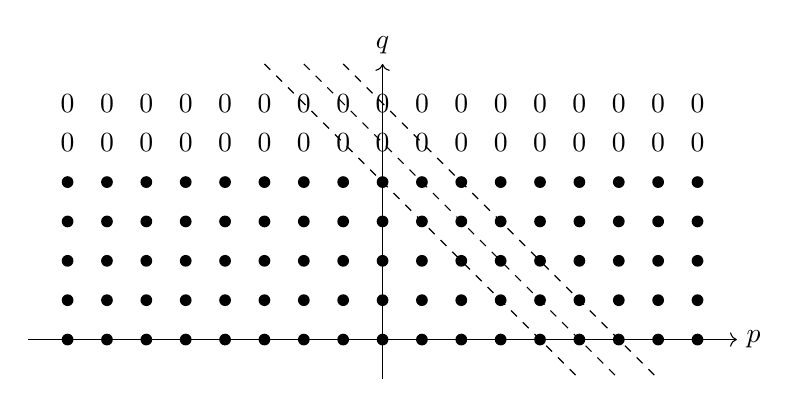
\begin{tikzpicture}[x=0.5cm, y=0.5cm]
        \draw[dashed] (-3,7) -- (5,-1);
        \draw[dashed] (-2,7) -- (6,-1);
        \draw[dashed] (-1,7) -- (7,-1);

        \draw[->] (0,-1) -- (0,7) node[above] {$q$};
        \draw[->] (-9,0) -- (9,0) node[right] {$p$};

        \foreach \p in {-8, ..., 8}
        \foreach \q in {5, ..., 6}
        \draw (\p,\q) node {$0$};

        \foreach \p in {-8, ..., 8}
        \foreach \q in {0, ..., 4}
        \draw (\p,\q) node[circle,fill,inner sep=1.5pt] {};
      \end{tikzpicture}
    \end{center}

    \noindent where all objects are \emph{finite} $2$-torsion.
  \end{proof}
\end{lemma}

\begin{lemma}
  \label{lemma:RGammac(GR,X(C),Z(n))-almost-perfect}
  The complex $R\Gamma_c (G_\RR, X (\CC), \ZZ (n))$
  is almost perfect.

  \begin{proof}
    Similarly, we consider the spectral sequence
    \[ E_2^{pq} = H^p (G_\RR, H^q_c (X (\CC), \ZZ (n)))
    \Longrightarrow
    H^{p+q}_c (G_\RR, X (\CC), \ZZ (n)). \]

    Here $H^p (G_\RR, H^q_c (X (\CC), \ZZ (n)))$ is not necessarily $2$-torsion
    for $p = 0$, and the second page looks like
    \begin{center}
      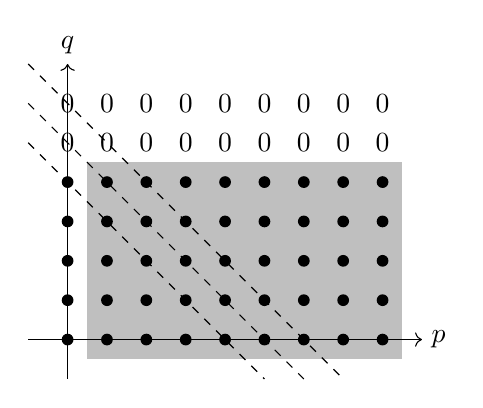
\begin{tikzpicture}[x=0.5cm, y=0.5cm]
        \fill[lightgray] (0.5,-0.5) -- (0.5,4.5) -- (8.5,4.5) -- (8.5,-0.5) -- cycle;

        \draw[dashed] (-1,5) -- (5,-1);
        \draw[dashed] (-1,6) -- (6,-1);
        \draw[dashed] (-1,7) -- (7,-1);

        \draw[->] (0,-1) -- (0,7) node[above] {$q$};
        \draw[->] (-1,0) -- (9,0) node[right] {$p$};

        \foreach \p in {0, ..., 8}
        \foreach \q in {5, ..., 6}
        \draw (\p,\q) node {$0$};

        \foreach \p in {0, ..., 8}
        \foreach \q in {0, ..., 4}
        \draw (\p,\q) node[circle,fill,inner sep=1.5pt] {};
      \end{tikzpicture}
    \end{center}
    where the shaded part $E_2^{pq}$, $p > 0$ consists of finitely generated
    $2$-torsion groups, the line $E_2^{0q}$ consists of finitely generated
    groups, and the objects $E_2^{pq}$ are zero for $q \gg 0$. It follows that
    the groups $H^i (G_\RR, X (\CC), \ZZ (n))$ are all finitely generated as
    well, and they are torsion for $i \gg 0$. This is in fact $2$-torsion, and
    we may see this as follows. If $P_\bullet \twoheadrightarrow \ZZ$ is the
    bar-resolution of $\ZZ$ by free $\ZZ G_\RR$-modules, then the morphism of
    complexes
    \[ \begin{tikzcd}
      \cdots\ar{r} & P_3\ar{r}\ar{d}{2} & P_2\ar{r}\ar{d}{2} & P_1\ar{r}\ar{d}{2} & P_0\ar{r}\ar{d}{2-N} & 0 \\
      \cdots\ar{r} & P_3\ar{r} & P_2\ar{r} & P_1\ar{r} & P_0\ar{r} & 0
    \end{tikzcd} \]

    \begin{align*}
      \text{``}2\text{''}\colon P_\bullet & \to P_\bullet,\\
      (2-N)\colon P_0 & \to P_0,\\
      2\colon P_i & \to P_i \quad\text{for }i > 1,
    \end{align*}
    which induces multiplication by $2$ on $H^i (G,-)$ for $i > 0$
    is null-homotopic \cite[Theorem 6.5.8]{Weibel-1994}. It is not
    multiplication by $2$ in degree $0$, but as the complex
    $R\Gamma_c (G_\RR, X (\CC), \ZZ (n))$ is bounded, we see that it induces
    multiplication by $2$ on $H^i (G_\RR, X (\CC), \ZZ (n))$ for $i \gg 0$.
  \end{proof}
\end{lemma}

Similarly for $\QQ/\ZZ$-coefficients, we have the following observation.

\begin{lemma}
  \label{lemma:RGammac(GR,X(C),Q/Z(n))-almost-cofinite-type}
  The complex $R\Gamma_c (G_\RR, X (\CC), \QQ/\ZZ (n))$
  is almost of cofinite type.

  \begin{proof}
    Consider the spectral sequence
    \[ E_2^{pq} = H^p (G_\RR, H^q_c (X (\CC), \QQ/\ZZ (n)))
    \Longrightarrow
    H^{p+q} (G_\RR, X (\CC), \QQ/\ZZ (n)). \]

    The second page will have groups of cofinite type on the line $E_2^{0q}$ and
    finite $2$-torsion groups $E_2^{pq}$ for $p > 0$. We have filtrations
    \begin{equation}
      \label{eqn:ss-filtrations}
      H^{p+q} = F^0 (H^{p+q}) \supseteq
      F^1 (H^{p+q}) \supseteq
      F^2 (H^{p+q}) \supseteq \cdots \supseteq
      F^{p+q} (H^{p+q}) \supset F^{p+q+1} (H^{p+q}) = 0
    \end{equation}
    where
    $$0 \to F^{p+1} (H^{p+q}) \to F^p (H^{p+q}) \to E_\infty^{pq} \to 0$$
    Note that $E^{0q}_\infty$ will be groups of cofinite type, and
    $E^{pq}_\infty$ will be finite $2$-torsion groups for $p > 0$, as we are
    going to have
    $$0 \to E_{r+1}^{0q} \to E_r^{0q} \to T \to 0$$
    where $T$ is finite $2$-torsion, and similarly,
    $$E_{r+1}^{pq} \cong \ker d_r^{pq} / \im d_r^{p-r,q+r-1}$$

    \[ E_r^{p-r,q+r-1} \xrightarrow{d_r^{p-r,q+r-1}}
    E_r^{pq} \xrightarrow{d_r^{pq}} E_r^{p+r,q-r+1} \]
    where $E_r^{pq}$ is finite $2$-torsion for $p > 0$. It follows by induction
    that all the members of the filtration \eqref{eqn:ss-filtrations} are finite
    groups, except for $F^0 (H^{p+q}) = H^{p+q}$ itself, which is of cofinite
    type, being an extension of a group of cofinite type $E_\infty^{0q}$ by a
    finite group $F^1 (H^{p+q})$
    (see Lemma~\ref{lemma:extensions-of-cofinite-type-groups}).
    We also see that $H^{p+q}$ is $2$-torsion for $p+q \gg 0$.
  \end{proof}
\end{lemma}

%%%%%%%%%%%%%%%%%%%%%%%%%%%%%%%%%%%%%%%%%%%%%%%%%%%%%%%%%%%%%%%%%%%%%%%%%%%%%%%%

\section{An arithmetic duality theorem}
\label{sec:arithmetic-duality-theorem}

At the heart of our constructions is a certain arithmetic duality theorem for
cycle complexes obtained by Thomas Geisser in \cite{Geisser-2010}. The goal of
this section is to deduce the following result from Geisser's duality.

\begin{theorem}
  \label{thm:duality}
  Assuming the conjecture $\mathbf{L}^c (X_\et,n)$, there is a quasi-isomorphism
  of complexes
  \[ R\widehat{\Gamma}_c (X_\et, \ZZ (n)) \xrightarrow{\cong}
  \RHom (R\Gamma (X_\et, \ZZ^c (n)), \QQ/\ZZ [-2]). \]
  In particular, the cohomology of
  $R\widehat{\Gamma}_c (X_\et, \ZZ (n))$ is of cofinite type.
\end{theorem}

Here $R\widehat{\Gamma}_c (X_\et, \ZZ (n))$ denotes the modified étale
cohomology with compact support, which is reviewed in the appendix
\ref{app:modified-cohomology-with-compact-support}. We note that
\cite{Geisser-2010} uses the notation ``$R\Gamma_c$'' for our
``$R\widehat{\Gamma}_c$'', but we take extra care to distinguish the two things,
as we will also need the usual étale cohomology with compact support
$R\Gamma_c (X_\et, \ZZ (n))$.

We split our proof of Theorem~\ref{thm:duality} in two propositions.

\begin{proposition}
  For any $n < 0$ we have a quasi-isomorphism of complexes
  \begin{equation}
    \label{eqn:duality-quasi-isomorphism-1}
    R\widehat{\Gamma}_c (X_\et, \ZZ (n)) \cong
    \varinjlim_m \RHom (R\Gamma (X_\et, \ZZ/m\ZZ^c (n)), \QQ/\ZZ [-2]).
  \end{equation}

  \begin{proof}
    We unwind our definition of $\ZZ (n)$ for $n < 0$ and reduce everything to
    the results from \cite{Geisser-2010}.

    \vspace{1em}

    As we have
    $\ZZ (n) \dfn \bigoplus_p \varinjlim_r j_{p!} \mu_{p^r}^{\otimes n} [-1]$,
    it will be enough to show that for every prime $p$ and $r=1,2,3,\ldots$
    there is a quasi-isomorphism of complexes
    \[ R\widehat{\Gamma}_c (X_\et, j_{p!} \mu_{p^r}^{\otimes n} [-1]) \cong
    \RHom (R\Gamma (X_\et, \ZZ^c/p^r (n)), \QQ/\ZZ [-2]), \]
    and then pass to the corresponding filtered colimits.

    As in the Definition~\ref{dfn:sheaf-Z(n)}, here $j_p$ denotes the canonical
    open immersion $j_p\colon X[1/p] \hookrightarrow X$. We further denote by
    $f$ the structure morphism $X\to \Spec \ZZ$ and by $f_p$ the structure
    morphism $X [1/p] \to \Spec \ZZ [1/p]$:

    \[ \begin{tikzcd}
      X [1/p]\ar[hookrightarrow]{r}{j_p}\ar{d}[swap]{f_p} & X\ar{d}{f} \\
      \Spec \ZZ [1/p]\ar[hookrightarrow]{r} & \Spec \ZZ
    \end{tikzcd} \]

    As we are going to change the base scheme, let us write $\Hom_X (-,-)$ for
    the $\Hom$ between sheaves on $X_\et$ and $\iHom_X (-,-)$ for the
    internal $\Hom$. Instead of $\Hom_{\Spec R}$, we will simply write
    $\Hom_R$.

    By \cite[Proposition 7.10, (c)]{Geisser-2010}, we have the following
    exchange formulas. If we work with complexes of constructible sheaves on the
    étale site of schemes over the spectrum of a number ring
    $\Spec\mathcal{O}$, then for a morphism $\phi$ of such schemes we have
    \begin{align}
      \label{eqn:exchange-formua-1} R \phi_* \mathcal{D} (\mathcal{F}) & \cong \mathcal{D} (R \phi_! \mathcal{F}),\\
      \label{eqn:exchange-formua-2} R \phi^! \mathcal{D} (\mathcal{G}) & \cong \mathcal{D} (\phi^* \mathcal{G}),
    \end{align}
    where the dualization is given by
    \[ \mathcal{D} (\mathcal{F}^\bullet) \dfn
    R\iHom_X (\mathcal{F}^\bullet, \ZZ^c (0)). \]

    Applying the exchange formula \eqref{eqn:exchange-formua-1} to our
    situation, we get
    \begin{equation}
      R\iHom_X (j_{p!} \mu_{p^r}^{\otimes n} [-1], \ZZ^c_X (0)) \cong
      R j_{p*} R\iHom_{X [1/p]} (\mu_{p^r}^{\otimes n} [-1], \ZZ^c_{X [1/p]} (0)).
    \end{equation}

    Using the other exchange formula \eqref{eqn:exchange-formua-2}, we may
    identify the sheaf
    $R\iHom_{X [1/p]} (\mu_{p^r}^{\otimes n} [-1], \ZZ^c_{X [1/p]} (0))$:
    \begin{align}
      \label{eqn:inverse-image-of-mu} R\iHom_{X [1/p]} (\mu_{p^r}^{\otimes n} [-1], \ZZ^c_{X [1/p]} (0)) & \cong R\iHom_{X[1/p]} (f_p^* \mu_{p^r}^{\otimes n} [-1], \ZZ^c_{X [1/p]} (0)) \\
      \label{eqn:exchange-formula-applied} & \cong R f^!_p R\iHom_{\ZZ [1/p]} (\mu_{p^r}^{\otimes n} [-1], \ZZ^c_{\ZZ [1/p]} (0)) \\
      \label{eqn:identification-of-Zc0-with-Gm} & \cong R f^!_p R\iHom_{\ZZ [1/p]} (\mu_{p^r}^{\otimes n} [-1], \mathbb{G}_\mathrm{m} [1]) \\
      & \cong R f^!_p R\iHom_{\ZZ [1/p]} (\mu_{p^r}^{\otimes n}, \mathbb{G}_\mathrm{m}) [2] \\
      & \cong R f^!_p \mu_{p^r}^{\otimes (1-n)} [2]
    \end{align}

    Here \eqref{eqn:inverse-image-of-mu} simply means that the sheaf
    $\mu_{p^r}^{\otimes n}$ on $X[1/p]$ is the same as the inverse image of the
    corresponding sheaf on $\Spec \ZZ [1/p]$. The quasi-isomorphism
    \eqref{eqn:exchange-formula-applied} is the first exchange formula. Then,
    \eqref{eqn:identification-of-Zc0-with-Gm} is the fact that the complex
    $\ZZ^c_{\ZZ [1/p]} (0)$ is quasi-isomorphic to $\mathbb{G}_\mathrm{m} [1]$
    according to \cite[Lemma 7.4]{Geisser-2010}. Thanks to
    \cite[Theorem 1.2]{Geisser-2004}, we may identify the sheaf
    $\mu_{p^r}^{\otimes (1-n)}$:
    \begin{equation}
      \mu_{p^r}^{\otimes (1-n)} \cong \ZZ_{\ZZ [1/p]}/p^r (1-n) =
      \ZZ^c_{\ZZ [1/p]}/p^r (n) [-2].
    \end{equation}

    Then \cite[Corollary 7.9]{Geisser-2010} tells us that
    \begin{equation}
      R f^!_p \ZZ^c_{\ZZ [1/p]} / p^r (n) \cong \ZZ^c_{X [1/p]} / p^r (n).
    \end{equation}

    Finally, thanks to \cite[Theorem 7.2 (a)]{Geisser-2010} and
    \cite[Proposition 2.3]{Geisser-2010}, we have
    $\ZZ^c_{X [1/p]}/p^r (n) \cong j_p^*\ZZ^c_X/p^r (n)$, and all the above
    gives
    \begin{equation}
      R\iHom_X (j_{p!} \mu_{p^r}^{\otimes n} [-1], \ZZ^c_X (0)) \cong
      R j_{p*} j_p^* \ZZ^c_X/p^r (n) \cong \ZZ^c_X/p^r (n).
    \end{equation}

    After applying $R\Gamma (X_\et, -)$, we get a quasi-isomorphism of
    complexes of abelian groups
    \begin{equation}
      \RHom (j_{p!} \mu_{p^r}^{\otimes n} [-1], \ZZ^c_X (0)) \cong
      R\Gamma (X_\et, \ZZ^c_X/p^r (n)).
    \end{equation}

    Now according to the duality theorem \cite[Theorem 7.8]{Geisser-2010},
    we have
    \begin{equation}
      \RHom (j_{p !} \mu_{p^r}^{\otimes n} [-1], \ZZ^c (0)) \cong
      \RHom (R\widehat{\Gamma}_c (X_\et, j_{p !} \mu_{p^r}^{\otimes n} [-1]), \QQ/\ZZ [-2]).
    \end{equation}

    So what we obtain at the end is a quasi-isomorphism
    \[ R\Gamma (X_\et, \ZZ^c/p^r (n)) \cong
    \RHom (R\widehat{\Gamma}_c (X_\et, j_{p !} \mu_{p^r}^{\otimes n} [-1]), \QQ/\ZZ [-2]). \]
    This is almost what we need: if we apply $\RHom (-,\QQ/\ZZ [-2])$, then, as
    $\widehat{H}^i_c (X_\et, j_{p!} \mu_{p^r}^{\otimes n} [-1])$ are
    finite groups (because the sheaves $j_{p!} \mu_{p^r}^{\otimes n}$ are
    constructible), we have
    \begin{multline*}
      \RHom (R\Gamma (X_\et, \ZZ^c/p^r (n)), \QQ/\ZZ[-2]) \cong\\
      \RHom (\RHom (R\widehat{\Gamma}_c (X_\et, j_{p !} \mu_{p^r}^{\otimes n} [-1]), \QQ/\ZZ[-2]), \QQ/\ZZ[-2]) \\
      \cong R\widehat{\Gamma}_c (X_\et, j_{p !} \mu_{p^r}^{\otimes n} [-1]). \qedhere
    \end{multline*}
  \end{proof}
\end{proposition}

Now to conclude the proof of Theorem~\ref{thm:duality}, we identify the complex
on the right hand side of \eqref{eqn:duality-quasi-isomorphism-1}. For this we
will need the conjecture $\mathbf{L}^c (X_\et, n)$.

\begin{proposition}
  \label{prop:a-quasi-isomorphism-with-dirlim}
  Assuming the conjecture $\mathbf{L}^c (X_\et, n)$, there is
  a quasi-isomorphism of complexes
  \[ \varinjlim_m \RHom (R\Gamma (X_\et, \ZZ/m\ZZ^c (n)), \QQ/\ZZ [-2]) \cong
  \RHom (R\Gamma (X_\et, \ZZ^c (n)), \QQ/\ZZ [-2]). \]

  \begin{proof}
    As $\ZZ^c (n)$ is a complex of flat sheaves, the short exact sequence of
    abelian groups
    $$0 \to \ZZ \xrightarrow{\times m} \ZZ \to \ZZ/m\ZZ \to 0$$
    induces a short exact sequence of sheaves
    \begin{equation}
      \label{short-exact-sequence-with-Z/m}
      0 \to \ZZ^c (n) \xrightarrow{\times m} \ZZ^c (n) \to \ZZ/m\ZZ^c (n) \to 0
    \end{equation}

    The morphism $\ZZ^c (n) \to \ZZ/m\ZZ^c (n)$ induces some morphisms in
    cohomology
    $$H^i (X_\et, \ZZ^c (n)) \to H^i (X_\et, \ZZ/m\ZZ^c (n)).$$

    We claim that if we pass to the duals $\Hom (-, \QQ/\ZZ)$ and then to the
    filtered colimits $\varinjlim_m$, then we obtain an isomorphism. (Note that
    both $\Hom (-, \QQ/\ZZ)$ and $\varinjlim_m$ are exact.)

    The short exact sequence \eqref{short-exact-sequence-with-Z/m} induces
    a long exact sequence in cohomology
    \[ \begin{tikzcd}[column sep=1em,font=\small]
      \cdots\ar{r} & H^i (X_\et, \ZZ^c (n)) \ar{r}{\times m} & H^i (X_\et, \ZZ^c (n))\ar{r} \ar[draw=none]{d}[name=X, anchor=center]{} & H^i (X_\et, \ZZ/m\ZZ^c (n)) \ar[rounded corners,to path={ -- ([xshift=2ex]\tikztostart.east) |- (X.center) \tikztonodes -| ([xshift=-2ex]\tikztotarget.west) -- (\tikztotarget)}]{dll}[at end]{\delta^i} \\
      & H^{i+1} (X_\et, \ZZ^c (n)) \ar{r}{\times m} & H^{i+1} (X_\et, \ZZ^c (n))\ar{r} & H^{i+1} (X_\et, \ZZ/m\ZZ^c (n)) \ar{r} & \cdots
    \end{tikzcd} \]

    We further have exact sequences
    \[ \begin{tikzcd}[row sep=0.8em,column sep=1em,font=\small]
      & & & \ker \delta^i\ar[equal]{d} \\
      & H^i (X_\et, \ZZ^c (n)) \ar{r}{\times m} & H^i (X_\et, \ZZ^c (n))\ar{r} & H^i (X_\et, \ZZ^c (n))_m \ar{r} & 0 \\
      0\ar{r} & {}_m H^{i+1} (X_\et, \ZZ^c (n)) \ar{r} & H^{i+1} (X_\et, \ZZ^c (n))\ar{r}{\times m} & H^{i+1} (X_\et, \ZZ^c (n)) \\
      & \im \delta^i\ar[equal]{u}
    \end{tikzcd} \]
    that give us
    \[ 0 \to H^i (X_\et, \ZZ^c (n))_m \to
    H^i (X_\et, \ZZ/m\ZZ^c (n)) \to
    {}_m H^{i+1} (X_\et, \ZZ^c (n)) \to 0 \]
    Now if we take $\Hom (-,\QQ/\ZZ)$ and filtered colimits $\varinjlim_m$,
    we get
    \begin{multline}
      \label{eqn:short-exact-sequence-with-dirlim}
      0 \to \varinjlim_m \Hom ({}_m H^{i+1} (X_\et, \ZZ^c (n)), \QQ/\ZZ) \to \\
      \varinjlim_m \Hom (H^i (X_\et, \ZZ/m\ZZ^c (n)), \QQ/\ZZ) \to
      \varinjlim_m \Hom (H^i (X_\et, \ZZ^c (n))_m, \QQ/\ZZ) \to 0
    \end{multline}

    By the conjecture $\mathbf{L}^c (X_\et, n)$, the group
    $H^{i+1} (X_\et, \ZZ^c (n))$ is finitely generated, and therefore
    the first $\varinjlim_m$ in the short exact sequence
    \eqref{eqn:short-exact-sequence-with-dirlim} vanishes, and we obtain
    isomorphisms
    \[ \varinjlim_m \Hom (H^i (X_\et, \ZZ^c (n))_m, \QQ/\ZZ) \xrightarrow{\cong}
    \varinjlim_m \Hom (H^i (X_\et, \ZZ/m\ZZ^c (n)), \QQ/\ZZ). \]
    It remains to note that the first $\varinjlim_m$ above is canonically
    isomorphic to $\Hom (H^i (X_\et, \ZZ^c (n)), \QQ/\ZZ)$, again,
    thanks to finite generation of $H^i (X_\et, \ZZ^c (n))$,
    assuming the conjecture $\mathbf{L}^c (X_\et, n)$.
  \end{proof}
\end{proposition}

We note that the conjecture $\mathbf{L}^c (X_\et, n)$ actually implies that the
complex $R\Gamma (X_\et, \ZZ^c (n))$ is bounded.

\begin{lemma}
  \label{lemma:RGamma(Xet,Zc(n))-perfect}
  Assuming the conjecture $\mathbf{L}^c (X_\et, n)$, the complex
  $R\Gamma (X_\et, \ZZ^c (n))$ is perfect.

  \begin{proof}
    First we claim that
    $$H^i (X_\et, \ZZ^c (n)) = 0\quad\text{for }i < -2\,\dim X.$$
    The complex of sheaves $\ZZ^c (n)$ is flat, so the short exact sequence of
    abelian groups
    $$0 \to \ZZ \to \QQ \to \QQ/\ZZ \to 0$$
    gives us a short exact sequence of étale sheaves
    $$0 \to \ZZ^c (n) \to \QQ^c (n) \to \QQ/\ZZ^c (n) \to 0$$
    and then applying $R\Gamma (X_\et, -)$, we obtain a distinguished
    triangle in $\mathbf{D} (\ZZ)$
    \[ R\Gamma (X_\et, \ZZ^c (n)) \to
    R\Gamma (X_\et, \QQ^c (n)) \to
    R\Gamma (X_\et, \QQ/\ZZ^c (n)) \to
    R\Gamma (X_\et, \ZZ^c (n)) [1] \]
    Now according to \cite[Lemma~5.12]{Morin-2014} (note that the proof there
    also uses Geisser's duality theorem), we have
    $$H^i (X_\et, \QQ/\ZZ^c (n)) = 0 \quad\text{for }i < -2\,\dim X,$$
    and the above triangle implies that
    \[ H^i (X_\et, \QQ^c (n)) \cong
    H^i (X_\et, \ZZ^c (n)) \quad\text{for }i < -2\,\dim X. \]
    However, $H^i (X_\et, \QQ^c (n))$ is a $\QQ$-vector space, and
    according to the conjecture $\mathbf{L}^c (X_\et, n)$, the groups
    $H^i (X_\et, \ZZ^c (n))$ are finitely generated over $\ZZ$. This
    means that for $i < -2\,\dim X$ these groups are trivial.

    Now to see that $H^i (X_\et, \ZZ^c (n)) = 0$ for $i \gg 0$, note that the
    duality theorem~\ref{thm:duality} gives
    \[ \widehat{H}_c^i (X_\et, \ZZ (n)) \cong
    \Hom (H^{2-i} (X_\et, \ZZ^c (n)), \QQ/\ZZ), \]
    where $H^{2-i} (X_\et, \ZZ^c (n))$ is a finitely generated group by our
    conjecture and $\widehat{H}_c^i (X_\et, \ZZ (n)) = 0$ for $i \ll 0$.
  \end{proof}
\end{lemma}

\begin{lemma}
  \label{lemma:morphism-hat-Hc(Xet,Z(n))->Hc(Xet,Z(n))}
  The canonical morphism
  $\widehat{H}^i_c (X_\et, \ZZ (n)) \to H^i_c (X_\et, \ZZ (n))$
  sits in a long exact sequence
  \[ \cdots \to \widehat{H}^{i-1}_c (G_\RR, X (\CC), \ZZ (n)) \to
  \widehat{H}_c^i (X_\et, \ZZ(n)) \to
  H_c^i (X_\et, \ZZ(n)) \to
  \widehat{H}^i_c (G_\RR, X (\CC), \ZZ (n)) \to \cdots \]
  where the groups $\widehat{H}^i_c (G_\RR, X (\CC), \ZZ (n))$ are finite
  $2$-torsion.  In particular, the kernel and cokernel of
  $\widehat{H}^i_c (X_\et, \ZZ (n)) \to H^i_c (X_\et, \ZZ (n))$ is finite
  $2$-torsion.

  \begin{proof}
    The exact sequence follows from the definition of modified étale cohomology
    with compact support and Artin's comparison theorem. This is done in
    \cite[Lemma~6.14]{Flach-Morin-2018}.
    The fact that $\widehat{H}^i_c (G_\RR, X (\CC), \ZZ (n))$ are finite
    $2$-torsion is Lemma~\ref{lemma:H-hat-c-GR-X(C)-Z(n)-finite-2-torsion}.
  \end{proof}
\end{lemma}

\begin{lemma}
  \label{lemma:RGammac(Xet,Z(n))-almost-cofinite-type}
  Assuming the conjecture $\mathbf{L}^c (X_\et,n)$, the complexes
  \[ R\widehat{\Gamma}_c (X_\et, \ZZ (n)), ~
  R\widehat{\Gamma}_c (X_\et, \QQ/\ZZ (n)), \quad
  \text{(resp. }
  R\Gamma_c (X_\et, \ZZ (n)), ~
  R\Gamma_c (X_\et, \QQ/\ZZ (n))\text{).} \]
  are of cofinite type (resp. almost of cofinite type) in the sense of
  \ref{dfn:almost-of-(co)finite-type}.

  \begin{proof}
    Recall that by the definition, $\ZZ (n) = \QQ/\ZZ (n) [-1]$.
    By Lemma~\ref{lemma:RGamma(Xet,Zc(n))-perfect}, the conjecture
    $\mathbf{L}^c (X_\et,n)$ implies that $R\Gamma (X_\et, \ZZ^c (n))$ is a
    perfect complex, and by Theorem~\ref{thm:duality} we have
    \[ R\widehat{\Gamma}_c (X_\et, \ZZ (n)) \cong
    \RHom (R\Gamma (X_\et, \ZZ^c (n)), \QQ/\ZZ [-2]), \]
    so that $R\widehat{\Gamma}_c (X_\et, \ZZ (n))$ is of cofinite type.

    As for $R\Gamma_c (X_\et, \ZZ (n))$, we have
    $H^i_c (X_\et, \ZZ (n)) \cong \widehat{H}^i_c (X_\et, \ZZ (n))$
    up to some finite $2$-torsion according to
    Lemma~\ref{lemma:morphism-hat-Hc(Xet,Z(n))->Hc(Xet,Z(n))}.
  \end{proof}
\end{lemma}

%%%%%%%%%%%%%%%%%%%%%%%%%%%%%%%%%%%%%%%%%%%%%%%%%%%%%%%%%%%%%%%%%%%%%%%%%%%%%%%%

\section{Complexes $R\Gamma_\fg (X, \ZZ(n))$}
\label{sec:RGamma-fg}

\begin{definition}
  Assuming the conjecture $\mathbf{L}^c (X_\et,n)$, consider a morphism
  $\alpha_{X,n}$ in the derived category $\mathbf{D} (\ZZ)$ given by the
  composition
  \[ \begin{tikzcd}[column sep=4em]
    \RHom (R\Gamma (X_\et, \ZZ^c (n)), \QQ[-2]) \ar{r}{\QQ \twoheadrightarrow \QQ/\ZZ}\ar{ddr}[swap]{\alpha_{X,n}} & \RHom (R\Gamma (X_\et, \ZZ^c (n)), \QQ/\ZZ[-2]) \\
    & R\widehat{\Gamma}_c (X_\et, \ZZ (n)) \ar{u}{\text{Theorem \ref{thm:duality}}}[swap]{\cong} \ar{d}{\text{proj.}} \\
    & R\Gamma_c (X_\et, \ZZ (n))
  \end{tikzcd} \]

  Here the first arrow is induced by the canonical projection $\QQ \to \QQ/\ZZ$,
  and the last arrow is the canonical projection from the modified cohomology
  with compact support to the usual cohomology with compact support
  (see Appendix~\ref{app:modified-cohomology-with-compact-support}).

  We define the complex $R\Gamma_\fg (X, \ZZ(n))$ as a cone of $\alpha_{X,n}$:
  \[ \RHom (R\Gamma (X_\et, \ZZ^c (n)), \QQ [-2]) \xrightarrow{\alpha_{X,n}}
  R\Gamma_c (X_\et, \ZZ (n)) \to
  R\Gamma_\fg (X, \ZZ(n)) \to
  \RHom (R\Gamma (X_\et, \ZZ^c (n)), \QQ [-1]) \]
\end{definition}

\vspace{1em}

We note that our $R\Gamma_\fg (X, \ZZ (n))$ plays the same role as
$R\Gamma_W (\overline{X}_\et, \ZZ (n))$ that appears in
\cite[Definition~3.6]{Flach-Morin-2018}. We use a different notation, since
Flach and Morin work with Artin--Verdier topology and their complex
$R\Gamma_W (\overline{X}_\et, \ZZ (n))$ is perfect, while for our complex
$H^i_\fg (X, \ZZ (n))$ may be finite $2$-torsion in arbitrarily high degree.

We first note that although the definition might seem complicated at first,
it simplifies if $X$ has no real places.

\begin{proposition}
  \label{prop:RGamma-fg-for-X(R)-empty}
  If $X (\RR) = \emptyset$, then
  \[ R\Gamma_\fg (X, \ZZ (n)) \cong
  \RHom (R\Gamma (X_\et, \ZZ^c (n)), \ZZ [-1]). \]

  \begin{proof}
    In this case
    $R\widehat{\Gamma}_c (X_\et, \ZZ (n)) \to R\Gamma_c (X_\et, \ZZ (n))$
    is the identity morphism
    (see Appendix~\ref{app:modified-cohomology-with-compact-support}),
    and therefore $\alpha_{X,n}$ sits in the following commutative diagram with
    exact columns:
    \[ \begin{tikzcd}
      \RHom (R\Gamma (X_\et, \ZZ^c (n)), \QQ [-2])\ar{d}{\alpha_{X,n}} \ar{r}{\mathrm{id}} & \RHom (R\Gamma (X_\et, \ZZ^c (n)), \QQ [-2])\ar{d} \\
      R\Gamma_c (X_\et, \ZZ (n))\ar{d} \ar{r}{\cong}[swap]{\text{Theorem \ref{thm:duality}}} & \RHom (R\Gamma (X_\et, \ZZ^c (n)), \QQ/\ZZ [-2])\ar{d} \\
      R\Gamma_\fg (X, \ZZ (n))\ar{d} \ar[dashed]{r}{\cong} & \RHom (R\Gamma (X_\et, \ZZ^c (n)), \ZZ [-1])\ar{d} \\
      \RHom (R\Gamma (X_\et, \ZZ^c (n)), \QQ [-1]) \ar{r}{\mathrm{id}} & \RHom (R\Gamma (X_\et, \ZZ^c (n)), \QQ [-1])
    \end{tikzcd} \]
    Here the first column is our definition of $R\Gamma_\fg (X, \ZZ (n))$,
    and the second column is induced by the distinguished triangle
    $\ZZ \to \QQ \to \QQ/\ZZ \to \ZZ [1]$.
  \end{proof}
\end{proposition}

\begin{proposition}
  \label{prop:RGammafg-almost-perfect}
  The complex $R\Gamma_\fg (X, \ZZ (n))$ is almost perfect in the
  sense of \ref{dfn:almost-of-(co)finite-type}, i.e. its cohomology groups
  $H^i_\fg (X, \ZZ (n)) \dfn H^i (R\Gamma_\fg (X, \ZZ (n)))$
  are finitely generated, trivial for $i \ll 0$, and only have $2$-torsion for
  $i \gg 0$.

  \begin{proof}
    By the definition of $R\Gamma_\fg (X, \ZZ (n))$, we have a long exact
    sequence
    \[ \begin{tikzcd}[column sep=1.75em]
      \cdots\ar{r} & \Hom (H^{2-i} (X_\et, \ZZ^c (n)), \QQ) \ar{r}{H^i (\alpha_{X,n})} &[2em] H^i_c (X_\et, \ZZ (n))\ar{r}\ar[draw=none]{d}[name=X, anchor=center]{} & H^i_\fg (X, \ZZ (n)) \ar[rounded corners,to path={ -- ([xshift=2ex]\tikztostart.east) |- (X.center) \tikztonodes -| ([xshift=-2ex]\tikztotarget.west) -- (\tikztotarget)}]{dll}[at end]{\delta^i} \\
      & \Hom (H^{1-i} (X_\et, \ZZ^c (n)), \QQ)\ar{r}{H^{i+1} (\alpha_{X,n})} & H^{i+1}_c (X_\et, \ZZ (n))\ar{r} & \cdots
    \end{tikzcd} \]

    First we observe from this that for $i \ll 0$ we have
    $\widehat{H}_c^i (X_\et, \ZZ(n)) = H_c^i (X_\et, \ZZ(n)) = 0$, and then
    \[ H^i_\fg (X, \ZZ(n)) \cong \Hom (H^{1-i} (X_\et, \ZZ^c (n)), \QQ)
    = 0 \quad\text{by Lemma~\ref{lemma:RGamma(Xet,Zc(n))-perfect}}. \]
    Similarly, for $i \gg 0$ holds $H^{2-i} (X_\et, \ZZ^c (n)) = 0$
    thanks to Lemma~\ref{lemma:RGamma(Xet,Zc(n))-perfect}, and therefore
    \[ H^i_\fg (X, \ZZ (n)) \cong H^i_c (X_\et, \ZZ(n))
    = \text{finite }2\text{-torsion by Lemma~\ref{lemma:RGammac(Xet,Z(n))-almost-cofinite-type}}. \]

    Now we consider short exact sequences
    \[ \begin{tikzcd}[row sep=0.5em]
      0 \ar{r} & \ker \delta^i \ar{r}\ar[equals]{d} & H^i_\fg (X, \ZZ (n)) \ar{r} & \im \delta^i \ar{r}\ar[equals]{d} & 0\\
      & \coker H^i (\alpha_{X,n}) & & \ker H^{i+1} (\alpha_{X,n})
    \end{tikzcd} \]

    By the definition of $\alpha_{X,n}$, the morphism $H^i (\alpha_{X,n})$ factors as
    \[ \Hom (H^{2-i} (X_\et, \ZZ^c (n)), \QQ) \to
    \Hom (H^{2-i} (X_\et, \ZZ^c (n)), \QQ/\ZZ) \xrightarrow{\cong}
    \widehat{H}^i_c (X_\et, \ZZ (n)) \to H^i_c (X_\et, \ZZ (n)) \]

    We recall from Lemma~\ref{lemma:morphism-hat-Hc(Xet,Z(n))->Hc(Xet,Z(n))}
    that the morphism $\widehat{H}^i_c (X_\et, \ZZ (n)) \to H^i_c (X_\et, \ZZ
    (n))$ has finite $2$-torsion kernel and cokernel.

    The group $H^{2-i} (X_\et, \ZZ^c (n))$ is finitely generated
    according to the conjecture $\mathbf{L}^c (X_\et, n)$. If this
    group is of the form $\ZZ^{\oplus r}\oplus T$, the morphism
    $H^i (\alpha_{X,n})$ is given by
    $$\QQ^{\oplus r} \twoheadrightarrow (\QQ/\ZZ)^{\oplus r} \rightarrowtail \widehat{H}^i_c (X_\et, \ZZ (n)) \to H^i_c (X_\et, \ZZ (n))$$
    where
    $(\QQ/\ZZ)^{\oplus r} \rightarrowtail \widehat{H}^i_c (X_\et, \ZZ (n))$ is
    the inclusion of the maximal divisible subgroup in the group of cofinite
    type
    $$\widehat{H}^i_c (X_\et, \ZZ (n)) \cong \Hom (H^{2-i} (X_\et, \ZZ^c (n)), \QQ/\ZZ).$$
    Both kernel and cokernel of the above map are finitely generated, hence
    $H^i_\fg (X, \ZZ (n))$ is finitely generated.
  \end{proof}
\end{proposition}

\begin{proposition}
  \label{prop:RGamma-fg-uniquely-defined}
  $R\Gamma_\fg (X, \ZZ (n))$ is defined up to a unique isomorphism in the
  derived category $\mathbf{D} (\ZZ)$.

  \begin{proof}
    The complex $\RHom (R\Gamma (X_\et, \ZZ^c (n)), \QQ [-2])$ consists of
    $\QQ$-vector spaces, and $R\Gamma_\fg (X, \ZZ (n))$ is almost perfect, so we
    are in the situation of \ref{TR3-TR1-with-uniqueness}.
  \end{proof}
\end{proposition}

\begin{proposition}
  \label{prop:tensoring-RGammafg-with-Z/m-and-Q}
   Consider a distinguished triangle defining $R\Gamma_\fg (X, \ZZ (n))$:
   \[ \RHom (R\Gamma (X_\et, \ZZ^c (n)), \QQ [-2]) \xrightarrow{\alpha_{X,n}}
   R\Gamma_c (X_\et, \ZZ (n)) \xrightarrow{f}
   R\Gamma_\fg (X, \ZZ (n)) \xrightarrow{g}
   \RHom (R\Gamma (X_\et, \ZZ^c (n)), \QQ [-1]) \]

   \begin{enumerate}
   \item[1)] For each $m = 1,2,3$ the morphism $f$ induces an isomorphism
     \[ f\otimes \ZZ/m\ZZ\colon
     R\Gamma_c (X_\et, \ZZ (n))\otimes_\ZZ^\mathbf{L} \ZZ/m\ZZ \xrightarrow{\cong}
     R\Gamma_\fg (X, \ZZ (n))\otimes_\ZZ^\mathbf{L} \ZZ/m\ZZ \]

   \item[2)] The morphism $g$ induces an isomorphism
     \[ g\otimes \QQ\colon R\Gamma_\fg (X, \ZZ (n)) \otimes_\ZZ \QQ \xrightarrow{\cong}
     \RHom (R\Gamma (X_\et, \ZZ^c (n)), \QQ [-1]).\]
   \end{enumerate}

   \begin{proof}
     The complexes $\RHom (R\Gamma (X_\et, \ZZ^c (n)), \QQ [\cdots])$ consist of
     $\QQ$-vector spaces, so they are killed by tensoring with
     $\ZZ/m\ZZ$. Similarly, the cohomology groups $H_c^i (X_\et, \ZZ (n))$ are
     all torsion, and therefore one has
     $R\Gamma_c (X_\et, \ZZ (n)) \otimes_\ZZ \QQ \cong 0$ in the derived
     category.
   \end{proof}
\end{proposition}

%%%%%%%%%%%%%%%%%%%%%%%%%%%%%%%%%%%%%%%%%%%%%%%%%%%%%%%%%%%%%%%%%%%%%%%%%%%%%%%%

\section{Weil-étale complexes $R\Gamma_\Wc (X, \ZZ(n))$}
\label{sec:RGamma-Wc}

The goal of this section is to construct Weil-étale cohomology complexes
$R\Gamma_\Wc (X, \ZZ(n))$.

\begin{definition}
  \label{dfn:u-infty}
  We define
  $v_\infty^*\colon R\Gamma_c (X_\et, \QQ/\ZZ (n)) \to R\Gamma_c (G_\RR, X (\CC), \QQ/\ZZ (n))$
  as the morphism in the derived category $\mathbf{D} (\ZZ)$ induced by the
  comparison of étale and analytic topology
  \[ \Gamma_c (X_\et, \QQ/\ZZ (n)) \to
  \Gamma_c (G_\RR, X (\CC), \alpha^* \QQ/\ZZ (n)) \cong
  \Gamma_c (G_\RR, X (\CC), \QQ/\ZZ (n)) \]
  (see \ref{prop:inverse-image-gamma} and \ref{propn:image-of-QZn-under-alpha}).
  
  Let
  $u_\infty^*\colon R\Gamma_c (X_\et, \ZZ(n)) \to R\Gamma_c (G_\RR, X (\CC), \ZZ (n))$
  be the composition
  \[ R\Gamma_c (X_\et, \ZZ(n)) \dfn R\Gamma_c (X_\et, \QQ/\ZZ (n)) [-1]
  \xrightarrow{v_\infty^* [-1]} R\Gamma_c (G_\RR, X (\CC), \QQ/\ZZ (n)) [-1] \to
  R\Gamma_c (G_\RR, X (\CC), \ZZ (n)) \]
  where the last arrow is induced by $\QQ/\ZZ (n) [-1] \to \ZZ (n)$, which comes
  from the distinguished triangle of constant $G_\RR$-equivariant sheaves
  $\ZZ (n) \to \QQ (n) \to \QQ/\ZZ (n) \to \ZZ (n) [1]$.
\end{definition}

The main result of this section is the following.

\begin{theorem}
  \label{thm:u-alpha-0}
  Let $X$ be an arithmetic scheme and $n < 0$. Assume the conjecture
  $\mathbf{L}^c (X_\et, n)$, so that the morphism $\alpha_{X,n}$ exists.
  Then $u_\infty^* \circ \alpha_{X,n} = 0$.

  \[ \begin{tikzcd}
    \RHom (R\Gamma (X, \ZZ^c (n)), \QQ [-2]) \ar{d}[swap]{\alpha_{X,n}}\ar{r} & 0\ar{d} \\
      R\Gamma_c (X_\et, \ZZ (n)) \ar{r}{u_\infty^*} & R\Gamma_c (G_\RR, X (\CC), \ZZ (n))
    \end{tikzcd} \]
\end{theorem}

This seems to be rather nontrivial; our argument (motivated by
\cite{Flach-Morin-2018} where it is given under the assumption that $X$ is
proper and regular) will be based on the following result about $\ell$-adic
cohomology.

\begin{proposition}
  \label{prop:l-adic-cohomology-key-lemma}
  Let $f\colon X\to \Spec \ZZ$ be an arithmetic scheme (that is, with $f$
  separated, of finite type). Let $n < 0$. Then for any prime $\ell$ we have
  $$(H^i_c (X_{\overline{\QQ},\text{\it ét}}, \QQ_\ell/\ZZ_\ell (n))^{G_\QQ})_{div} = 0.$$

  \begin{proof}
    Let us recall some facts about $\ell$-adic cohomology. We refer to
    \cite[Exposé~VI]{SGA5} for details. Let us first consider the sheaf
    $\ZZ_\ell (n)$. It is a
    \textbf{constructible $\ZZ_\ell$-sheaf}\footnote{Or simply
      \textbf{$\ZZ_\ell$-sheaf} in the terminology of \cite[Rapport]{SGA4-1-2}.}
    on $X$ in the sense of \cite[Exposé~VI, 1.1.1]{SGA5}. We would like to
    compare the cohomology of $\ZZ_\ell (n)$ on
    $X_{\overline{\QQ},\text{\it ét}}$ and $X_{\overline{\FF_p},\text{\it ét}}$,
    where $p$ is some prime different from $\ell$, to be determined later.
    For this we fix some algebraic closures $\overline{\QQ}/\QQ$ and
    $\overline{\FF_p}/\FF_p$ and consider the corresponding morphisms
    \[ \overline{\eta}\colon \Spec \overline{\QQ} \to \Spec \ZZ, \quad
    \overline{x}\colon \Spec \overline{\FF_p} \to \Spec \ZZ. \]
    Let $X_{\overline{\QQ},\text{\it ét}}$ and
    $X_{\overline{\FF_p},\text{\it ét}}$ be the pullbacks of $X$ along the above
    morphisms:
    \[ \begin{tikzcd}
      X_{\overline{\QQ}} \ar{r}\tikzpb\ar{d}[swap]{f_{\overline{\QQ}}} & X \ar{d}{f} & X_{\overline{\FF_p}} \ar{l}\ar{d}{f_{\overline{\FF_p}}}\tikzpbur \\
      \Spec \overline{\QQ} \ar{r}[swap]{\overline{\eta}} & \Spec \ZZ & \Spec \overline{\FF_p} \ar{l}{\overline{x}}
    \end{tikzcd} \]

    According to \cite[Exposé~VI, 2.2.3]{SGA5}, the proper base change theorem
    holds for constructible $\ZZ_\ell$-sheaves. It gives us isomorphisms
    \[ H^i_c (X_{\overline{\QQ}, \text{\it ét}}, \ZZ_\ell (n)) \cong (R^i f_! \ZZ_\ell (n))_{\overline{\eta}}, \quad
    H^i_c (X_{\overline{\FF_p}, \text{\it ét}}, \ZZ_\ell (n)) \cong (R^i f_! \ZZ_\ell (n))_{\overline{x}}, \]
    where $R^i f_! \ZZ_\ell (n)$ is the same sheaf on $\Spec \ZZ$, and we take
    its different stalks to get cohomology with compact support on different
    fibers. The construction of higher direct images with proper support
    $R^i f_! \mathcal{F}$ for $\ell$-adic sheaves is given in
    \cite[Exposé~VI, \S 2.2]{SGA5}. The key nontrivial fact that we need is that
    for every morphism (of locally noetherian schemes) $f\colon X\to Y$,
    separated of finite type, if $\mathcal{F}$ is a constructible
    $\ZZ_\ell$-sheaf on $X$, then $R^i f_! \mathcal{F}$ is a constructible
    $\ZZ_\ell$-sheaf on $Y$.

    According to \cite[Exposé~VI, 1.2.6]{SGA5}, for a projective system of
    abelian sheaves $\mathcal{F} = (\mathcal{F}_n)_{n\in\NN}$ on $X_\et$, the
    following are equivalent:
    \begin{enumerate}
    \item[1)] $\mathcal{F}$ is a constructible $\ZZ_\ell$-sheaf,

    \item[2)] every open subscheme $U\subset X$ is a finite union of locally
      closed pieces $Z_i$ where $\left.\mathcal{F}\right|_{Z_i}$ is a
      \textbf{twisted constant constructible $\ZZ_\ell$-sheaf}\footnote{A
        \textbf{faisceau lisse} in the terminology of
        \cite[Rapport]{SGA4-1-2}.}.
    \end{enumerate}

    Being ``twisted constant'' means that each sheaf $\mathcal{F}_n$ in the
    projective system $(\mathcal{F}_n)_{n\in\NN}$ is locally constant. The
    importance of twisted constant sheaves is explained by the following
    property \cite[Exposé~VI, 1.2.4, 1.2.5]{SGA5}: for a connected locally
    noetherian scheme $X$, the category of twisted constant
    $\ZZ_\ell$-constructible sheaves on $X$ is equivalent to the category of
    finitely generated $\ZZ_\ell$-modules with a continuous action of the étale
    fundamental group $\pi_1^\text{\it ét} (X)$.

    In our setting, all this means that there exists an open subscheme
    $$U = \Spec \ZZ_S \subset \Spec \ZZ,$$
    where $\ZZ_S$ denotes the localization of $\ZZ$ at a finite set of primes
    $S$, such that the sheaves $R^i f_! \ZZ_\ell (n)$ are twisted constant on
    $U$. By removing all the necessary bad primes, we can make sure this holds
    for all $i$.

    Now there exists some prime $p \notin S$ (that is, $(p) \in U$), for which
    we may consider the following picture:
    \[ \begin{tikzcd}
      X_{\overline{\QQ}} \ar{r}\tikzpb\ar{d}[swap]{f_{\overline{\QQ}}} & X_U \ar{d}{f_U} & X_{\overline{\FF_p}} \ar{l}\ar{d}{f_{\overline{\FF_p}}}\tikzpbur \\
      \Spec \overline{\QQ} \ar{r}[swap]{\overline{\eta}} & U & \Spec \overline{\FF_p} \ar{l}{\overline{x}}
    \end{tikzcd} \]

    It follows that we have isomorphisms
    \begin{equation}
      \label{eqn:iso-pbc-Zl-Gal(QS/Q)}
      H^i_c (X_{\overline{\QQ}, \text{\it ét}}, \ZZ_\ell (n)) \cong (R^i f_{U,!} \ZZ_\ell (n))_{\overline{\eta}} \cong (R^i f_{U,!} \ZZ_\ell (n))_{\overline{x}} \cong H^i_c (X_{\overline{\FF_p}, \text{\it ét}}, \ZZ_\ell (n)),
    \end{equation}
    of finitely generated $\ZZ_\ell$-modules with continuous action of
    $$\pi_1^\text{\it ét} (U) \cong \Gal (\QQ_S/\QQ),$$
    where $\QQ_S/\QQ$ denotes a maximal extension of $\QQ$ unramified outside of
    $S$. We note that $(R^i f_{U,!} \ZZ_\ell (n))_{\overline{\eta}}$ naturally
    carries an action of $\pi_1^\text{\it ét} (U, \overline{\eta})$, while
    $(R^i f_{U,!} \ZZ_\ell (n))_{\overline{x}}$ carries an action of
    $\pi_1^\text{\it ét} (U, \overline{x})$, and the isomorphism in the middle
    of \eqref{eqn:iso-pbc-Zl-Gal(QS/Q)} sweeps under the rug an identification
    of $\pi_1^\text{\it ét} (U, \overline{\eta})$ with
    $\pi_1^\text{\it ét} (U, \overline{x})$.

    To state this more accurately, note that the $\ZZ_\ell$-module
    $H^i_c (X_{\overline{\QQ}, \text{\it ét}}, \ZZ_\ell (n))$ carries a natural
    action of $G_\QQ$ while $H^i_c (X_{\overline{\FF_p}, \text{\it ét}},
    \ZZ_\ell (n))$ carries a natural action of $G_{\FF_p}$. After making the
    necessary choices, we have $G_{\QQ_p} \subset G_\QQ$ and a short exact
    sequence
    $$1 \to I_p \to G_{\QQ_p} \to G_{\FF_p} \to 1$$
    where $I_p$ is the inertia subgroup, acting trivially on
    $H^i_c (X_{\overline{\QQ}, \text{\it ét}}, \ZZ_\ell (n))$. We have thus
    isomorphisms of finitely generated $\ZZ_\ell$-modules
    \[ H^i_c (X_{\overline{\QQ}, \text{\it ét}}, \ZZ_\ell (n)) \cong
    H^i_c (X_{\overline{\FF_p}, \text{\it ét}}, \ZZ_\ell (n)), \]
    equivariant under the action of $G_{\QQ_p}/I_p$ on the left hand side and of
    $G_{\FF_p}$ on the right hand side. To relate all this to $\QQ_\ell (n)$ and
    $\QQ_\ell/\ZZ_\ell (n)$-coefficients, note that we have the following
    isomorphic long exact sequences in cohomology
    \begin{equation}
      \label{eqn:Zl-Ql-Ql/Zl-les}
      \begin{tikzcd}[column sep=small, font=\small]
        \vdots \ar{d} & \vdots \ar{d} \\
        H_c^{i-1} (X_{\overline{\QQ},\text{\it ét}}, \QQ_\ell/\ZZ_\ell (n)) \ar{d}{\delta}\ar{r}{\cong} & H_c^{i-1} (X_{\overline{\FF_p},\text{\it ét}}, \QQ_\ell/\ZZ_\ell (n))  \ar{d}{\delta} \\
        H_c^i (X_{\overline{\QQ},\text{\it ét}}, \ZZ_\ell (n)) \ar{d}{\phi}\ar{r}{\cong} & H_c^i (X_{\overline{\FF_p},\text{\it ét}}, \ZZ_\ell (n)) \ar{d}{\phi} \\
        H_c^i (X_{\overline{\QQ},\text{\it ét}}, \QQ_\ell (n)) \ar{d}{\psi}\ar{r}{\cong} & H_c^i (X_{\overline{\FF_p},\text{\it ét}}, \QQ_\ell (n)) \ar{d}{\psi} \\
        H_c^i (X_{\overline{\QQ},\text{\it ét}}, \QQ_\ell/\ZZ_\ell (n)) \ar{r}\ar{d}{\cong} & H_c^i (X_{\overline{\FF_p},\text{\it ét}}, \QQ_\ell/\ZZ_\ell (n)) \ar{d} \\
        \vdots & \vdots \\
      \end{tikzcd}
\end{equation}

    Here
    \begin{align*}
      H_c^i (X_{\overline{\QQ},\text{\it ét}}, \QQ_\ell (n)) & = H_c^i (X_{\overline{\QQ},\text{\it ét}}, \ZZ_\ell (n))\otimes_{\ZZ_\ell} \QQ_\ell,\\
      H_c^i (X_{\overline{\FF_p},\text{\it ét}}, \QQ_\ell (n)) & = H_c^i (X_{\overline{\FF_p},\text{\it ét}}, \ZZ_\ell (n))\otimes_{\ZZ_\ell} \QQ_\ell,
    \end{align*}
    and the arrows $\phi$ above are canonical localization morphisms.
    The horizontal arrows are equivariant isomorphisms in the above sense. Note
    that we have
    \[ H^i_c (X_{\overline{\QQ}, \text{\it ét}}, \QQ_\ell/\ZZ_\ell (n))^{G_\QQ} \rightarrowtail
    H^i_c (X_{\overline{\QQ}, \text{\it ét}}, \QQ_\ell/\ZZ_\ell (n))^{G_{\QQ_p}/I_p}
    \cong H^i_c (X_{\overline{\FF_p}, \text{\it ét}}, \QQ_\ell/\ZZ_\ell (n))^{G_{\FF_p}}, \]
    so in order to prove that
    $$(H^i_c (X_{\overline{\QQ},\text{\it ét}}, \QQ_\ell/\ZZ_\ell (n))^{G_\QQ})_{div} = 0,$$
    it will be enough to show that
    $$(H^i_c (X_{\overline{\FF_p},\text{\it ét}}, \QQ_\ell/\ZZ_\ell (n))^{G_{\FF_p}})_{div} = 0.$$
    From now on we move to the characteristic $p$ and consider the fixed points
    of $G_{\FF_p}$ acting on the $\ZZ_\ell$-module
    $H^i_c (X_{\overline{\FF_p},\text{\it ét}}, \QQ_\ell/\ZZ_\ell (n))$.
    In the long exact sequence \eqref{eqn:Zl-Ql-Ql/Zl-les}, we have (keeping in
    mind that $\phi$ is merely the localization morphism):
    \begin{align*}
      \ker \phi & = H^i_c (X_{\overline{\FF_p},\text{\it ét}}, \ZZ_\ell (n))_{tor},\\
      \ker \psi & = \im \phi \cong H^i_c (X_{\overline{\FF_p},\text{\it ét}}, \ZZ_\ell (n)) / \ker \phi \\
      & \quad\quad\quad = \frac{H^i_c (X_{\overline{\FF_p},\text{\it ét}}, \ZZ_\ell (n))}{H^i_c (X_{\overline{\FF_p},\text{\it ét}}, \ZZ_\ell (n))_{tor}} \rdfn H^i_c (X_{\overline{\FF_p},\text{\it ét}}, \ZZ_\ell (n))_{cotor},\\
      \im \psi & = H_c^i (X_{\overline{\FF_p},\text{\it ét}}, \QQ_\ell/\ZZ_\ell (n))_{div}.
    \end{align*}

    This gives us a short exact sequence
    \[ 0 \to H^i_c (X_{\overline{\FF_p},\text{\it ét}}, \ZZ_\ell (n))_{cotor} \to
    H^i_c (X_{\overline{\FF_p},\text{\it ét}}, \QQ_\ell (n)) \to
    H^i_c (X_{\overline{\FF_p},\text{\it ét}}, \QQ_\ell/\ZZ_\ell (n))_{div} \to 0 \]
    After taking the $G_{\FF_p}$-invariants, we obtain a long exact sequence
    of cohomology groups
    \begin{multline}
      \label{eqn:cohomology-long-exact-sequence-with-GFp}
      0 \to (H^i_c (X_{\overline{\FF_p},\text{\it ét}}, \ZZ_\ell (n))_{cotor})^{G_{\FF_p}} \to
      H^i_c (X_{\overline{\FF_p},\text{\it ét}}, \QQ_\ell (n))^{G_{\FF_p}} \\
      \to (H^i_c (X_{\overline{\FF_p},\text{\it ét}}, \QQ_\ell/\ZZ_\ell (n))_{div})^{G_{\FF_p}} \to
      H^1 (G_{\FF_p}, H^i_c (X_{\overline{\FF_p},\text{\it ét}}, \ZZ_\ell (n))_{cotor}) \to \cdots
    \end{multline}

    We claim that
    \begin{equation}
      \label{eqn:SGA-7-expose-XXI-5-5-3}
      H^i_c (X_{\overline{\FF_p},\text{\it ét}}, \QQ_\ell (n))^{G_{\FF_p}} = 0.
    \end{equation}

    Indeed, according to \cite[Exposé~XXI, 5.5.3]{SGA7}, the eigenvalues of the
    geometric Frobenius acting on
    $H^i_c (X_{\overline{\FF_p},\text{\it ét}}, \QQ_\ell)$ are algebraic
    integers. We are twisting $\QQ_\ell$ by $n$, so the eigenvalues of Frobenius
    lie in $p^{-n}\,\overline{\ZZ}$. Since $n < 0$ by our assumption, this
    implies that $1$ does not occur as an eigenvalue.

    Now \eqref{eqn:SGA-7-expose-XXI-5-5-3} and the long exact sequence
    \eqref{eqn:cohomology-long-exact-sequence-with-GFp} imply that there is a
    monomorphism
    \[ (H^i_c (X_{\overline{\FF_p},\text{\it ét}}, \QQ_\ell/\ZZ_\ell (n))_{div})^{G_{\FF_p}} \rightarrowtail
    H^1 (G_{\FF_p}, H^i_c (X_{\overline{\FF_p},\text{\it ét}}, \ZZ_\ell (n))_{cotor}), \]
    which restricts to a monomorphism between the maximal divisible subgroups
    \[ ((H^i_c (X_{\overline{\FF_p},\text{\it ét}}, \QQ_\ell/\ZZ_\ell (n))_{div})^{G_{\FF_p}})_{div} \rightarrowtail
    H^1 (G_{\FF_p}, H^i_c (X_{\overline{\FF_p},\text{\it ét}}, \ZZ_\ell (n))_{cotor})_{div}. \]
    However,
    $H^1 (G_{\FF_p}, H^i_c (X_{\overline{\FF_p},\text{\it ét}}, \ZZ_\ell (n))_{cotor})$
    is a finitely generated $\ZZ_\ell$-module, and therefore its
    maximal divisible subgroup is trivial. We have therefore
    \[ (H^i_c (X_{\overline{\FF_p},\text{\it ét}}, \QQ_\ell/\ZZ_\ell (n))^{G_{\FF_p}})_{div} =
    ((H^i_c (X_{\overline{\FF_p},\text{\it ét}}, \QQ_\ell/\ZZ_\ell (n))_{div})^{G_{\FF_p}})_{div} = 0. \]
    (For the first equality, note that for any $G$-module $A$ one has
    $((A_{div})^G)_{div} = (A^G)_{div}$.)
  \end{proof}
\end{proposition}

\begin{proof}[Now we are ready to prove Theorem~\ref{thm:u-alpha-0}]
  The morphism $\alpha_{X,n}$ is defined on
  $$\RHom (R\Gamma (X_\et, \ZZ^c (n)), \QQ [-2]),$$
  which is a complex of $\QQ$-vector spaces, so it will be enough to show that
  $v_\infty^*$ is a torsion element in the abelian group
  $$\Hom_{\mathbf{D} (\ZZ)} (R\Gamma_c (X_\et, \QQ/\ZZ (n)), \, R\Gamma_c (G_\RR, X (\CC), \QQ/\ZZ (n))).$$

  The complexes $R\Gamma_c (X_\et, \QQ/\ZZ (n))$ and
  $R\Gamma_c (G_\RR, X (\CC), \QQ/\ZZ (n))$ are almost of cofinite type by
  Lemma~\ref{lemma:RGammac(Xet,Z(n))-almost-cofinite-type} and
  \ref{lemma:RGammac(GR,X(C),Q/Z(n))-almost-cofinite-type} respectively.
  Therefore, according to \ref{lemma:torsion-morphisms-in-D(Z)}, to show that
  $v^*_\infty\colon R\Gamma_c (X_\et, \QQ/\ZZ (n)) \to R\Gamma_c (G_\RR, X (\CC), \QQ/\ZZ (n))$
  is torsion in $\mathbf{D} (\ZZ)$, it is enough to show that the corresponding
  morphisms on the maximal divisible subgroups
  \[ H^i_c (v^*_\infty)_{div}\colon H^i_c (X_\et, \QQ/\ZZ (n))_{div} \to
  H^i_c (G_\RR, X (\CC), \QQ/\ZZ (n))_{div} \]
  are all trivial. The morphism $H^i_c (v^*_\infty)$ factors through
  $H^i_c (X_{\overline{\QQ}, \text{\it ét}}, \mu^{\otimes n})^{G_\QQ}$, where
  $\mu^{\otimes n}$ is the sheaf of all roots of unity on
  $X_{\overline{\QQ}, \text{\it ét}}$ twisted by $n$.
  We have therefore
  \[ \begin{tikzcd}[column sep=0pt]
    H^i_c (X_\et, \QQ/\ZZ (n))_{div}\ar{rr}{H^i_c (v^*_\infty)_{div}}\ar[dashed]{dr} && H^i_c (G_\RR, X (\CC), \QQ/\ZZ (n))_{div}\\
    & \left(H^i_c (X_{\overline{\QQ}, \text{\it ét}}, \mu^{\otimes n})^{G_\QQ}\right)_{div}\ar[dashed]{ur}
  \end{tikzcd} \]
  Now
  \[ \left(H^i_c (X_{\overline{\QQ}, \text{\it ét}}, \mu^{\otimes n})^{G_\QQ}\right)_{div} \cong
  \left(\bigoplus_\ell H^i_c (X_{\overline{\QQ}, \text{\it ét}}, \QQ_\ell/\ZZ_\ell (n))^{G_\QQ}\right)_{div} \cong
  \bigoplus_\ell \left(H^i_c (X_{\overline{\QQ}, \text{\it ét}}, \QQ_\ell/\ZZ_\ell (n))^{G_\QQ}\right)_{div}, \]
  where all summands are trivial according to
  \ref{prop:l-adic-cohomology-key-lemma}.
\end{proof}

\begin{definition}
  Let
  $i_\infty^*\colon R\Gamma_\fg (X, \ZZ (n)) \to R\Gamma_c (G_\RR, X (\CC), \ZZ (n))$
  be a morphism in $\mathbf{D} (\ZZ)$ that gives a morphism of distinguished
  triangles
  \begin{equation}
    \label{eqn:triangle-defining-i-infty}
    \begin{tikzcd}
      \RHom (R\Gamma (X, \ZZ^c (n)), \QQ [-2]) \ar{d}[swap]{\alpha_{X,n}}\ar{r} & 0\ar{d} \\
      R\Gamma_c (X_\et, \ZZ (n)) \ar{r}{u_\infty^*}\ar{d} &  R\Gamma_c (G_\RR, X (\CC), \ZZ (n)) \ar{d}{id} \\
      R\Gamma_\fg (X, \ZZ (n)) \ar[dashed]{r}{i_\infty^*}\ar{d} & R\Gamma_c (G_\RR, X (\CC), \ZZ (n)) \ar{d} \\
      \RHom (R\Gamma (X, \ZZ^c (n)), \QQ [-1])\ar{r} & 0 \\
    \end{tikzcd}
  \end{equation}
\end{definition}

\begin{proposition}
  \label{prop:uniqueness-of-i-infty}
  The morphism $i_\infty^*$ is uniquely defined.

  \begin{proof}
    We may apply \ref{TR3-TR1-with-uniqueness}, because
    $\RHom (R\Gamma (X, \ZZ^c (n)), \QQ [-2])$ is a complex of $\QQ$-vector
    spaces and both
    $R\Gamma_\fg (X, \ZZ (n))$ and
    $R\Gamma_c (G_\RR, X (\CC), \ZZ (n))$
    are almost perfect complexes by
    Proposition~\ref{prop:RGammafg-almost-perfect} and
    Lemma~\ref{lemma:RGammac(GR,X(C),Z(n))-almost-perfect}.
  \end{proof}
\end{proposition}

\begin{proposition}
  \label{i-infty-is-torsion}
  The morphism $i_\infty^*$ is torsion in the derived category,
  i.e. $i_\infty^*\otimes \QQ = 0$.

  \begin{proof}
    Let us examine the morphism of distinguished triangles
    \eqref{eqn:triangle-defining-i-infty} that defines $i_\infty^*$; in
    particular, the commutative diagram
    \[ \begin{tikzcd}
      R\Gamma_c (X_\et, \ZZ (n)) \ar{r}\ar{d}[swap]{u_\infty^*} & R\Gamma_\fg (X, \ZZ (n))\ar{dl}{i_\infty^*} \\
      R\Gamma_c (G_\RR, X (\CC), \ZZ (n))
    \end{tikzcd} \]

    According to \ref{TR3-TR1-with-uniqueness}, the morphism
    \[ \Hom_{\mathbf{D} (\ZZ)} (R\Gamma_\fg (X,\ZZ (n)), R\Gamma_c (G_\RR, X (\CC), \ZZ (n))) \to
    \Hom_{\mathbf{D} (\ZZ)} (R\Gamma_c (X_\et, \ZZ (n)), R\Gamma_c (G_\RR, X (\CC), \ZZ (n))) \]
    induced by the composition with
    $R\Gamma_c (X_\et, \ZZ (n)) \to R\Gamma_\fg (X,\ZZ (n))$, is mono, and
    therefore
    \begin{multline*}
      \Hom_{\mathbf{D} (\ZZ)} (R\Gamma_\fg (X,\ZZ (n)), R\Gamma_c (G_\RR, X (\CC), \ZZ (n)))\otimes_\ZZ \QQ \to\\
      \Hom_{\mathbf{D} (\ZZ)} (R\Gamma_c (X_\et, \ZZ (n)), R\Gamma_c (G_\RR, X (\CC), \ZZ (n)))\otimes_\ZZ \QQ
    \end{multline*}
    is mono as well. However, we just saw in the proof of \ref{thm:u-alpha-0}
    that $u_\infty^*\otimes \QQ = 0$, and this implies that
    $i_\infty^*\otimes \QQ = 0$.
  \end{proof}
\end{proposition}

Now we are ready to define Weil-étale complexes.

\begin{definition}
  \label{dfn:RGammaWc}
  $R\Gamma_\Wc (X,\ZZ(n))$ is an object in the derived category
  $\mathbf{D} (\ZZ)$ which is a mapping fiber of $i_\infty^*$:
  \[ R\Gamma_\Wc (X,\ZZ(n)) \to
  R\Gamma_\fg (X, \ZZ (n)) \xrightarrow{i_\infty^*}
  R\Gamma_c (G_\RR, X (\CC), \ZZ (n)) \to
  R\Gamma_\Wc (X,\ZZ(n)) [1] \]
  The \textbf{Weil-étale cohomology with compact support} is given by
  $$H_\Wc^i (X, \ZZ (n)) \dfn H^i (R\Gamma_\Wc (X,\ZZ(n))).$$
\end{definition}

\begin{remark}
  Note that this defines $R\Gamma_\Wc (X,\ZZ(n))$ up to a non-unique isomorphism
  in $\mathbf{D} (\ZZ)$, and the groups $H_\Wc^i (X, \ZZ (n))$ are also defined
  up to a non-unique isomorphism. In a continuation of this paper we will make
  use of the determinant $\det\nolimits_\ZZ R\Gamma_\Wc (X,\ZZ(n))$ (in the
  sense of \cite{Knudsen-Mumford-1976}), which will be defined up to a canonical
  isomorphism.

  Nevertheless, we recall from Proposition~\ref{prop:RGamma-fg-uniquely-defined}
  that $R\Gamma_\fg (X, \ZZ (n))$ is defined up to a unique isomorphism in the
  derived category $\mathbf{D} (\ZZ)$. If we could define
  $i_\infty^*\colon R\Gamma_\fg (X, \ZZ(n)) \to R\Gamma_c (G_\RR, X(\CC), \ZZ(n))$
  as an explicit, genuine morphism of complexes (not merely a morphism in the
  derived category $\mathbf{D} (\ZZ)$), this would give us a canonical and
  functorial definition for $R\Gamma_\Wc (X, \ZZ(n))$.
\end{remark}

\begin{proposition}
  \label{prop:RGammaWc-perfect}
  The conjecture $\mathbf{L}^c (X_\et, n)$ implies that $R\Gamma_\Wc (X,\ZZ(n))$
  is a perfect complex.

  \begin{proof}
    By definition, we have a long exact sequence in cohomology
    \[ \cdots \to H^{i-1}_c (G_\RR, X (\CC), \ZZ (n)) \to
    H^i_\Wc (X,\ZZ(n)) \to
    H^i_\fg (X,\ZZ(n)) \xrightarrow{H^i (i_\infty^*)}
    H^i_c (G_\RR, X (\CC), \ZZ (n)) \to \cdots \]

    The groups $H^i_c (G_\RR, X (\CC), \ZZ (n))$ and $H^i_\fg (X, \ZZ(n))$ are
    finitely generated by Lemma~\ref{lemma:RGammac(GR,X(C),Z(n))-almost-perfect}
    and Proposition~\ref{prop:RGammafg-almost-perfect}. They vanish for
    $i \ll 0$, but they are finite $2$-torsion for $i \gg 0$. I claim that
    $H^i (i_\infty^*)$ is an isomorphism for $i \gg 0$, meaning that this
    $2$-torsion in higher degrees does not appear in $H^i_\Wc (X,\ZZ(n))$.
    We have a commutative diagram
    \[ \begin{tikzcd}
      H^i_c (X_\et, \ZZ (n))\ar{r}\ar{d}[swap]{H^i (u_\infty^*)} & H^i_\fg (X, \ZZ (n))\ar{dl}{H^i (i_\infty^*)} \\
      H^i_c (G_\RR, X (\CC), \ZZ (n))
    \end{tikzcd} \]

    The morphism $H^i (u_\infty^*)$ is iso for $i \gg 0$, hence
    $H^i (i_\infty^*)$ is surjective for $i \gg 0$. However,
    $H^i_\fg (X, \ZZ (n))$ and $H^i_c (G_\RR, X (\CC), \ZZ (n))$ have the same
    $2$-torsion for $i \gg 0$, and $H^i (i_\infty^*)$ is iso for $i \gg 0$.
  \end{proof}
\end{proposition}

\begin{proposition}
  There is a non-canonical splitting
  \[ R\Gamma_\Wc (X, \ZZ(n)) \otimes_\ZZ \QQ \cong
  \RHom (R\Gamma (X_\et, \ZZ^c (n)), \QQ) [-1] \oplus
  R\Gamma_c (G_\RR, X (\CC), \QQ (n)) [-1]. \]

  \begin{proof}
    The distinguished triangle defining $R\Gamma_\Wc (X, \ZZ(n))$
    \[ R\Gamma_\Wc (X, \ZZ (n)) \to
    R\Gamma_\fg (X, \ZZ(n)) \xrightarrow{i_\infty^*}
    R\Gamma_c (G_\RR, X (\CC), \ZZ(n)) \to
    R\Gamma_\Wc (X, \ZZ (n)) [1] \]
    after tensoring with $\QQ$ becomes
    \[ R\Gamma_\Wc (X, \ZZ (n))\otimes_\ZZ \QQ \to
    R\Gamma_\fg (X, \ZZ(n))\otimes_\ZZ \QQ \xrightarrow{i_\infty^*\otimes\QQ = 0}
    R\Gamma_c (G_\RR, X (\CC), \ZZ(n))\otimes_\ZZ \QQ \to
    R\Gamma_\Wc (X, \ZZ (n))\otimes_\ZZ \QQ [1] \]
    which gives us a non-canonical splitting
    \cite[Chapitre~II, Corollaire~1.2.6]{Verdier-thesis}
    \[ R\Gamma_\Wc (X, \ZZ (n))\otimes_\ZZ \QQ \cong
    R\Gamma_\fg (X, \ZZ(n))\otimes_\ZZ \QQ \oplus
    R\Gamma_c (G_\RR, X (\CC), \ZZ(n)) [-1]\otimes_\ZZ \QQ, \]
    and we already noticed in \ref{prop:tensoring-RGammafg-with-Z/m-and-Q} that
    \[ R\Gamma_\fg (X, \ZZ (n)) \otimes_\ZZ \QQ \cong
    \RHom (R\Gamma (X_\et, \ZZ^c (n)), \QQ) [-1]. \qedhere \]
  \end{proof}
\end{proposition}

\begin{proposition}
  If the scheme $X$ is of characteristic $p$ (i.e. the morphism
  $X \to \Spec \ZZ$ factors through $\Spec \FF_p \to \Spec \ZZ$), then
  $$R\Gamma_\Wc (X,\ZZ(n)) \cong \RHom (R\Gamma (X_\et, \ZZ^c (n)), \ZZ [-1]).$$

  \begin{proof}
    Under our assumptions, $X (\CC) = X (\RR) = \emptyset$, and therefore
    $R\Gamma_c (G_\RR, X (\CC), \ZZ (n)) = 0$, so that
    $R\Gamma_\Wc (X,\ZZ(n)) \cong R\Gamma_\fg (X, \ZZ (n))$.
    Finally, according to \ref{prop:RGamma-fg-for-X(R)-empty}, we have
    an isomorphism
    $R\Gamma_\fg (X, \ZZ (n)) \cong \RHom (R\Gamma (X_\et, \ZZ^c (n)), \ZZ [-1])$.
  \end{proof}
\end{proposition}

%%%%%%%%%%%%%%%%%%%%%%%%%%%%%%%%%%%%%%%%%%%%%%%%%%%%%%%%%%%%%%%%%%%%%%%%%%%%%%%%

\pagebreak
\appendix
\section{Some homological algebra}
\label{app:homological-algebra}

This appendix collects some basic results about the derived category of abelian
groups $\mathbf{D} (\ZZ)$ that are used throughout the text. The lemmas below
are essentially isolated from \cite{Flach-Morin-2018}, with some modifications
to deal with $2$-torsion.

First we recall that every complex of abelian groups $A^\bullet$ is
quasi-isomorphic to its cohomology:
\[ A^\bullet \cong \bigoplus_{i\in \ZZ} H^i (A^\bullet) [-i] \cong
\prod_{i\in \ZZ} H^i (A^\bullet) [-i] =
\Bigl(\cdots \to H^{i-1} (A^\bullet) \xrightarrow{0} H^i (A^\bullet) \xrightarrow{0} H^{i+1} (A^\bullet) \to \cdots\Bigr). \]

This gives us a useful expression for morphisms in the derived category.
Since
\[ \Hom_{\mathbf{D} (\ZZ)} (A,B [i]) = \begin{cases}
\Hom_\ZZ (A,B), & i = 0,\\
\Ext_\ZZ^1 (A,B), & i = 1,\\
0, & \text{otherwise},
\end{cases} \]
we obtain
\begin{multline*}
  \Hom_{\mathbf{D} (\ZZ)} (A^\bullet, B^\bullet) \cong
  \Hom_{\mathbf{D} (\ZZ)} (\bigoplus_{i\in\ZZ} H^i (A^\bullet) [-i], \prod_{j\in\ZZ} H^j (B^\bullet) [-j]) \\
  \cong \prod_{i\in \ZZ} \prod_{j\in \ZZ} \Hom_{\mathbf{D} (\ZZ)} (H^i (A^\bullet), H^j (B^\bullet) [i-j]) \\
  \cong \prod_{i\in \ZZ} \left(\Hom_\ZZ (H^i (A^\bullet), H^i (B^\bullet)) \oplus \Ext_\ZZ^1 (H^i (A^\bullet), H^{i-1} (B^\bullet))\right).
\end{multline*}

Let us write down this formula for further reference:
\begin{equation}
  \label{eqn:morphisms-in-D(Z)}
  \Hom_{\mathbf{D} (\ZZ)} (A^\bullet, B^\bullet) \cong
  \prod_{i\in \ZZ} \Hom_\ZZ (H^i (A^\bullet), H^i (B^\bullet)) \oplus
  \prod_{i\in \ZZ} \Ext_\ZZ^1 (H^i (A^\bullet), H^{i-1} (B^\bullet)).
\end{equation}

\begin{lemma}
  \label{lemma:morphisms-inDAb-not-divisible}
  ~

  \begin{enumerate}
  \item[1)] If $C^\bullet$ and $C'^\bullet$ are almost perfect in the sense of
    Definition~\ref{dfn:almost-of-(co)finite-type}, then the group
    $\Hom_{\mathbf{D} (\ZZ)} (C^\bullet, C'^\bullet)$ has no nontrivial
    divisible subgroups.

  \item[2)] If $A^\bullet$ is a complex such that $H^i (A^\bullet)$ are finite
    dimensional $\QQ$-vector spaces and $C^\bullet$ is a complex such that
    $H^i (C^\bullet)$ are finitely generated abelian groups, then the group
    $\Hom_{\mathbf{D} (\ZZ)} (A^\bullet, C^\bullet)$ is divisible.
  \end{enumerate}

  \begin{proof}
    In 1), we consider the decomposition \eqref{eqn:morphisms-in-D(Z)} for
    $\Hom_{\mathbf{D} (\ZZ)} (C^\bullet, C'^\bullet)$, and observe that under
    our assumptions, both groups
    $\prod_{i\in\ZZ} \Hom_\ZZ (H^i (C^\bullet), H^i (C'^\bullet))$ and
    $\prod_{i\in\ZZ} \Ext_\ZZ^1 (H^i (C^\bullet), H^{i-1} (C'^\bullet))$ will be of
    the form $G \oplus T$, where $G$ is a finitely generated abelian group and
    $T$ is $2$-torsion. From this we see that if
    $x \in \Hom_{\mathbf{D} (\ZZ)} (C^\bullet, C'^\bullet)$ is divisible by all
    powers of $2$, then $x = 0$.

    Similarly, in part 2), we consider the decomposition
    \eqref{eqn:morphisms-in-D(Z)} for
    $\Hom_{\mathbf{D} (\ZZ)} (A^\bullet, C^\bullet)$. By our assumptions
    $\Hom_\ZZ (H^i (A^\bullet), H^i (C^\bullet)) = 0$ for all $i$, and each
    $\Ext_\ZZ^1 (H^i (A^\bullet), H^{i-1} (C^\bullet))$ is a direct sum of
    finitely many groups isomorphic to $\Ext_\ZZ^1 (\QQ,\ZZ)$, which is
    divisible. Therefore, $\Hom_{\mathbf{D} (\ZZ)} (A^\bullet, C^\bullet)$ is
    direct product of divisible groups, hence divisible.
  \end{proof}
\end{lemma}

Recall that Verdier's axiom (TR1) tells us that every morphism
$v\colon A^\bullet \to B^\bullet$ may be completed to a distinguished triangle
$A^\bullet \xrightarrow{u} B^\bullet \xrightarrow{v} C^\bullet \xrightarrow{w} A^\bullet [1]$.
The axiom (TR3) tells that for every commutative diagram with
distinguished rows
\begin{equation}
  \label{eqn:TR3-input}
  \begin{tikzcd}
    A^\bullet\ar{r}{u}\ar{d}{f} & B^\bullet\ar{r}{v}\ar{d}{g} & C^\bullet\ar{r}{w} & A^\bullet [1] \\
    A'^\bullet\ar{r}{u'} & B'^\bullet\ar{r}{v'} & C'^\bullet\ar{r}{w'} & A'^\bullet [1]
  \end{tikzcd}
\end{equation}
there exists some $h\colon C^\bullet \to C'^\bullet$ giving a morphism of
distinguished triangles
\begin{equation}
  \label{eqn:TR3-output}
  \begin{tikzcd}
    A^\bullet\ar{r}{u}\ar{d}{f} & B^\bullet\ar{r}{v}\ar{d}{g} & C^\bullet\ar{r}{w}\ar[dashed]{d}{\exists h} & A^\bullet [1]\ar{d}{f [1]} \\
    A'^\bullet\ar{r}{u'} & B'^\bullet\ar{r}{v'} & C'^\bullet\ar{r}{w'} & A'^\bullet [1]
  \end{tikzcd}
\end{equation}

The cone $C^\bullet$ in (TR1) and the morphism $h$ in (TR3) are neither unique
nor canonical. Two different cones of the same morphism are necessarily
isomorphic, but the isomorphism between them is not unique, because it is
provided by (TR3). This is a well-known issue with the derived category
formalism. Let us recall a useful standard argument which shows that at least in
some special cases, things are uniquely defined. The following is basically
\cite[Proposition~1.1.9, Corollaire~1.1.10]{Beilinson-Bernstein-Deligne}.

\begin{lemma}
  \label{TR3-TR1-with-uniqueness-general-statement}

  Consider the derived category $\mathbf{D} (\mathcal{A})$ of an abelian
  category $\mathcal{A}$.

  \begin{enumerate}
  \item[1)] For a commutative diagram \eqref{eqn:TR3-input}, assume that the
    homomorphism of abelian groups
    \[ w^*\colon \Hom_{\mathbf{D} (\mathcal{A})} (A^\bullet [1], C'^\bullet) \to
    \Hom_{\mathbf{D} (\mathcal{A})} (C^\bullet, C'^\bullet) \]
    induced by $w$ is trivial. Then there exists a unique morphism
    $h\colon C^\bullet \to C'^\bullet$ giving a morphism of triangles
    \eqref{eqn:TR3-output}.

  \item[2)] For a distinguished triangle
    $A^\bullet \xrightarrow{u} B^\bullet \xrightarrow{v} C^\bullet \xrightarrow{w} A^\bullet[1]$,
    assume that for any other cone $C'^\bullet$
    of $u$ the morphism $w^*$ is trivial. Then in fact the cone of $u$ is unique
    up to a unique isomorphism.
  \end{enumerate}

  \begin{proof}
    In 1), applying $\Hom_{\mathbf{D} (\mathcal{A})} (-, C'^\bullet)$ to the
    first distinguished triangle, we obtain an exact sequence of abelian groups
    \[ \Hom_{\mathbf{D} (\mathcal{A})} (A^\bullet [1], C'^\bullet) \xrightarrow{w^*}
    \Hom_{\mathbf{D} (\mathcal{A})} (C^\bullet, C'^\bullet) \xrightarrow{v^*}
    \Hom_{\mathbf{D} (\mathcal{A})} (B^\bullet, C'^\bullet). \]
    If $w^* = 0$, we conclude that $v^*$ is a monomorphism. This means that
    there is a unique morphism $h$ such that $h\circ v = v'\circ g$. Now in 2),
    if $C^\bullet$ and $C'^\bullet$ are two different cones of $u$, we have a
    commutative diagram
    \[ \begin{tikzcd}
      A^\bullet\ar{r}{u}\ar{d}{id} & B^\bullet\ar{r}{v}\ar{d}{id} & C^\bullet\ar{r}{w}\ar[dashed]{d} & A^\bullet [1]\ar{d}{id} \\
      A^\bullet\ar{r}{u'} & B^\bullet\ar{r}{v'} & C'^\bullet\ar{r}{w'} & A^\bullet [1]
    \end{tikzcd} \]
    As always, by the ``triangulated 5-lemma'', the dashed arrow is an
    isomorphism, and it is unique thanks to part 1).
  \end{proof}
\end{lemma}

Here is a particular case that we are going to use.

\begin{corollary}
  \label{TR3-TR1-with-uniqueness}
  Consider the derived category $\mathbf{D} (\ZZ)$.

  \begin{enumerate}
  \item[1)] Suppose we have a commutative diagram with distinguished rows
    \[ \begin{tikzcd}
    A^\bullet\ar{r}{u}\ar{d}{f} & B^\bullet\ar{r}{v}\ar{d}{g} & C^\bullet\ar{r}{w} & A^\bullet [1] \\
    A'^\bullet\ar{r}{u'} & B'^\bullet\ar{r}{v'} & C'^\bullet\ar{r}{w'} & A'^\bullet [1]
  \end{tikzcd} \]
    where $A^\bullet$ is a complex such that $H^i (A^\bullet)$ are finite
    dimensional $\QQ$-vector spaces and $C^\bullet$ and $C'^\bullet$ are almost
    perfect complexes in the sense of
    Definition~\ref{dfn:almost-of-(co)finite-type}. Then there exists a unique
    morphism ${h\colon C^\bullet \to C'^\bullet}$ giving a morphism of triangles
    \[ \begin{tikzcd}
      A^\bullet\ar{r}{u}\ar{d}{f} & B^\bullet\ar{r}{v}\ar{d}{g} & C^\bullet\ar{r}{w}\ar[dashed]{d}[d]{\exists ! h} & A^\bullet [1]\ar{d}{f [1]} \\
      A'^\bullet\ar{r}{u'} & B'^\bullet\ar{r}{v'} & C'^\bullet\ar{r}{w'} & A'^\bullet [1]
    \end{tikzcd} \]

  \item[2)] For a distinguished triangle
    $$A^\bullet \xrightarrow{u} B^\bullet \xrightarrow{v} C^\bullet \xrightarrow{w} A^\bullet[1]$$
    assume that $A^\bullet$ is a complex such that $H^i (A^\bullet)$ are finite
    dimensional $\QQ$-vector spaces and $C^\bullet$ is an almost perfect
    complex. Then the cone of $u$ is unique up to a unique isomorphism.
  \end{enumerate}

  \begin{proof}
    In this situation, according to \ref{lemma:morphisms-inDAb-not-divisible},
    the group $\Hom_{\mathbf{D} (\ZZ)} (C^\bullet, C'^\bullet)$ has no
    nontrivial divisible subgroups and
    $\Hom_{\mathbf{D} (\ZZ)} (A^\bullet [1], C'^\bullet)$ is divisible. This
    means that there are no nontrivial homomorphisms
    $\Hom_{\mathbf{D} (\ZZ)} (A^\bullet [1], C'^\bullet) \to \Hom_{\mathbf{D} (\ZZ)} (C^\bullet, C'^\bullet)$,
    and we may apply \ref{TR3-TR1-with-uniqueness-general-statement}.
  \end{proof}
\end{corollary}

\begin{lemma}
  \label{lemma:torsion-morphisms-in-D(Z)}
  Suppose that $A^\bullet$ and $B^\bullet$ are almost of cofinite type in the
  sense of Definition~\ref{dfn:almost-of-(co)finite-type}. Then a morphism
  $f\colon A^\bullet\to B^\bullet$ is torsion in $\mathbf{D} (\ZZ)$
  (i.e. a torsion element in the group
  $\Hom_{\mathbf{D} (\ZZ)} (A^\bullet, B^\bullet)$, i.e.
  $f\otimes \mathbb{Q} = 0$) if and only if the morphisms
  $$H^i (f)\colon H^i (A^\bullet) \to H^i (B^\bullet)$$
  are torsion, that is, they are trivial on the maximal divisible subgroups:
  $$(H^i (f)_{div}\colon H^i (A^\bullet)_{div} \to H^i (B^\bullet)_{div}) = 0.$$

  \begin{proof}
    In the formula \eqref{eqn:morphisms-in-D(Z)} the groups $H^i (A^\bullet)$
    and $H^{i-1} (B^\bullet)$ are of the form
    $(\mathbb{Q}/\mathbb{Z})^{\oplus r} \oplus T$, where $T$ is finite, and we
    calculate that
    \[ \Ext_\ZZ^1 ((\QQ/\ZZ)^{\oplus r} \oplus T, (\QQ/\ZZ)^{\oplus r'} \oplus T') \cong
    T'^{\oplus r} \oplus \Ext_\ZZ^1 (T, T') \]
    are finite groups.

    For $i \gg 0$, the groups $H^i (A^\bullet)$ and $H^{i-1} (B^\bullet)$ will
    be finite $2$-torsion, and therefore
    $\Ext_\ZZ^1 (H^i (A^\bullet), H^{i-1} (B^\bullet))$ will be finite
    $2$-torsion as well. It follows that the whole product
    $\prod_{i\in \mathbb{Z}} \Ext_\ZZ^1 (H^i (A^\bullet), H^{i-1} (B^\bullet))$
    is of the form $G \oplus T$, where $G$ is finite and $T$ is possibly
    infinite $2$-torsion. We have therefore $(G \oplus T)\otimes_\ZZ \QQ = 0$.

    Similarly, the group
    $\prod_{i\in\ZZ} \Hom_\ZZ (H^i (A^\bullet), H^i (B^\bullet))$ will consist
    of some part of the form $\widehat{\ZZ}^{\oplus r} \oplus G$, where $G$
    is finite, and some $2$-torsion part, which is killed by tensoring with
    $\QQ$. It follows that there is an isomorphism
    \begin{align*}
      \Hom_{\mathbf{D} (\ZZ)} (A^\bullet, B^\bullet)\otimes_\ZZ \mathbb{Q} & \cong
      \prod_{i\in \mathbb{Z}} \Hom_\ZZ (H^i (A^\bullet), H^i (B^\bullet)) \otimes_\ZZ \mathbb{Q}, \\
      f\otimes\QQ & \mapsto (H^i (f) \otimes \QQ)_{i\in\ZZ}. \qedhere
    \end{align*}
  \end{proof}
\end{lemma}

\begin{lemma}
  \label{lemma:morphisms-in-DAb-between-cplx-of-Q-vs-and-almost-cofinite-type-cplx}
  If $A^\bullet$ is a complex of $\QQ$-vector spaces and $B^\bullet$ is a
  complex almost of cofinite type in the sense of
  Definition~\ref{dfn:almost-of-(co)finite-type}, then there is an isomorphism
  of abelian groups
  \begin{align*}
    \Hom_{\mathbf{D} (\ZZ)} (A^\bullet, B^\bullet) & \xrightarrow{\cong}
    \prod_{i\in \ZZ} \Hom_\ZZ (H^i (A^\bullet), H^i (B^\bullet)),\\
    f & \mapsto (H^i (f))_{i\in \ZZ}.
  \end{align*}

  \begin{proof}
    In the formula \eqref{eqn:morphisms-in-D(Z)}, if $H^i (A^\bullet)$ are
    $\QQ$-vector spaces and $H^{i-1} (B^\bullet)$ have form
    $(\QQ/\ZZ)^{\oplus r} \oplus T$ with $T$ finite, we see that the summand with
    $\Ext_\ZZ^1 (H^i (A^\bullet), H^{i-1} (B^\bullet))$ vanishes.
  \end{proof}
\end{lemma}

%%%%%%%%%%%%%%%%%%%%%%%%%%%%%%%%%%%%%%%%%%%%%%%%%%%%%%%%%%%%%%%%%%%%%%%%%%%%%%%%

\pagebreak
\section{Cohomology with compact support}
\label{app:modified-cohomology-with-compact-support}

Let us first we recall the definition of étale cohomology with compact support.
For any arithmetic scheme $f\colon X\to \Spec \ZZ$ (separated, of finite type)
there exists a \textbf{Nagata compactification}
\[ \begin{tikzcd}
X \ar[hookrightarrow]{rr}{j}\ar{dr}[swap]{f} & & \mathfrak{X} \ar{dl}{g} \\
 & \Spec \ZZ
\end{tikzcd} \]
where $j$ is an open immersion and $g$ is a proper morphism. This is a result of
Nagata, and a modern exposition (following Deligne) may be found in
\cite{Conrad-Deligne-Nagata,Conrad-Deligne-Nagata-erratum}. See also
\cite[Exposé~XVII]{SGA4}.

\begin{definition}
  Let $X$ be an arithmetic scheme and let $\mathcal{F}$ be an abelian torsion
  sheaf on $X_\et$. Then one defines the
  \textbf{cohomology of $\mathcal{F}$ with compact support} via the complex
  \begin{equation}
    \label{eqn:RGammac-via-extension-by-zero}
    R\Gamma_c (X_\et, \mathcal{F}) \dfn
    R\Gamma (\mathfrak{X}_\text{\it \'et}, j_! \mathcal{F}).
  \end{equation}
\end{definition}

For torsion sheaves, this does not depend on the choice of
$j\colon X \hookrightarrow \mathfrak{X}$, but here we would like to fix this
choice to be able to compare cohomology with compact support on $X_\et$ with
the singular cohomology with compact support on $X (\CC)$.

\subsection*{Comparison with analytic cohomology}

\begin{definition}
  Given a Nagata compactification $j\colon X\hookrightarrow \mathfrak{X}$,
  we consider the corresponding open immersion
  $j (\CC)\colon X (\CC) \to \mathfrak{X} (\CC)$,
  and for a sheaf $\mathcal{F}$ on $X (\CC)$ we define
  \[ \Gamma_c (X (\CC), \mathcal{F}) \dfn
  \Gamma (\mathfrak{X} (\CC), j (\CC)_! \mathcal{F}). \]
  Similarly, for a $G_\RR$-equivariant sheaf on $X (\CC)$ we define
  \[ \Gamma_c (G_\RR, X (\CC), \mathcal{F}) \dfn
  \Gamma (G_\RR, \mathfrak{X} (\CC), j (\CC)_! \mathcal{F}). \]
\end{definition}

The canonical reference for comparison between étale and singular cohomology is
\cite[Exposé~XI, \S 4]{SGA4}, so let us to borrow some definitions and notation
from there. Let $X$ be an arithmetic scheme (separated, of finite type over
$\Spec \ZZ$).

\begin{enumerate}
\item The base change from $\Spec \ZZ$ to $\Spec \CC$ gives us a morphism of
  sites
  $\gamma\colon X_{\CC,\text{\it ét}} \to X_\et$.

\item As always, we denote by $X (\CC)$ the set of complex points of $X$
  equipped with the usual analytic topology.

  Let $X_\text{\it cl}$ be the site of étale maps $f\colon U\to X (\CC)$.
  A covering family in $X_\text{\it cl}$\footnote{``cl'' for ``classique''.}
  is a family of maps $\{ U_i \to U \}$ such that $U$ is the union of images of
  $U_i$.

  As the inclusion of an open subset $U \subset X (\CC)$ is trivially an étale
  map, we have a fully faithful functor $X (\CC) \subset X_\text{\it cl}$, and
  the topology on $X (\CC)$ is induced by the topology on
  $X_\text{\it cl}$. This gives us a morphism of sites
  $\delta\colon X_\text{\it cl} \to X (\CC)$,
  which by the well-known ``comparison lemma''
  \cite[Exposé~III, Théorème~4.1]{SGA4} induces an equivalence of the
  corresponding categories of sheaves
  $\delta_*\colon \mathbf{Sh} (X_\text{\it cl}) \to \mathbf{Sh} (X (\CC))$.

\item A morphism of schemes $f\colon X'_\CC \to X_\CC$ over $\Spec \CC$ is étale
  if and only if $f (\CC)\colon X' (\CC) \to X (\CC)$ is étale in the
  topological sense \cite[Exposé~XII, Proposition~3.1]{SGA1}, and therefore the
  functor $X'_\CC \rightsquigarrow X' (\CC)$ gives us a morphism of sites
  $\epsilon\colon X_\text{\it cl} \to X_{\CC,\text{\it ét}}$.
\end{enumerate}

We may now consider the composite functor
\[ \begin{tikzcd}
  \mathbf{Sh} (X_\et) \ar{r}{\gamma^*} &
  \mathbf{Sh} (X_{\CC,\text{\it ét}}) \ar{r}{\epsilon^*} &
  \mathbf{Sh} (X_\text{\it cl}) \ar{r}{\delta_*}[swap]{\simeq} &
  \mathbf{Sh} (X (\CC))
\end{tikzcd} \]
where $\gamma^*$ is given by the base change from $\Spec \ZZ$ to $\Spec \CC$,
the functor $\epsilon^*$ is the comparison, and $\delta_*$ is an equivalence of
categories. As we start from a scheme over $\Spec \ZZ$ and base change to
$\Spec \CC$, the resulting sheaf on $X (\CC)$ is in fact equivariant with
respect to the complex conjugation, and the above composition gives us an
``inverse image'' functor
$$\alpha^*\colon \mathbf{Sh} (X_\et) \to \mathbf{Sh} (G_\RR, X (\CC)).$$

\begin{proposition}
  \label{prop:inverse-image-gamma}
  Let $\mathcal{F}$ be a sheaf on $X_\et$.

  \begin{enumerate}
  \item[1)] There exists a natural morphism
    $$\Gamma (X_\et, \mathcal{F}) \to \Gamma (G_\RR, X (\CC), \alpha^* \mathcal{F}).$$

  \item[2)] Similarly for cohomology with compact support, there is a natural morphism
    $$\Gamma_c (X_\et, \mathcal{F}) \to \Gamma_c (G_\RR, X (\CC), \alpha^* \mathcal{F}).$$
  \end{enumerate}

  \begin{proof}
    This is standard and follows from the functoriality of $\alpha^*$.
    The morphism in 1) may be described as
    \begin{multline*}
      \Gamma (X_\et, \mathcal{F}) \xrightarrow{\cong} \Hom_{\mathbf{Sh} (X_\et)} (\underline{\{ \ast \}}, \mathcal{F}) \to
      \Hom_{\mathbf{Sh} (G_\RR, X (\CC))} (\alpha^*\underline{\{ \ast \}}, \alpha^* \mathcal{F}) \\
      \xrightarrow{\cong} \Hom_{\mathbf{Sh} (G_\RR, X (\CC))} (\underline{\{ \ast \}}, \alpha^* \mathcal{F}) \xrightarrow{\cong}
      \Gamma (G_\RR, X (\CC), \alpha^* \mathcal{F}).
    \end{multline*}

    For abelian sheaves, in the above formula one has to replace the constant
    sheaf $\underline{\{\ast\}}$ with $\underline{\ZZ}$. The naturality is
    easily seen from the above definition.

    In 2), if $j\colon X \hookrightarrow \mathfrak{X}$ is a Nagata
    compactification, then we have the corresponding compactification
    $j (\CC)\colon X (\CC) \hookrightarrow \mathfrak{X} (\CC)$. The extension by
    zero morphism
    $j (\CC)_!\colon \mathbf{Sh} (X (\CC)) \to \mathbf{Sh} (\mathfrak{X} (\CC))$
    restricts to the subcategory of $G_\RR$-equivariant sheaves:
    if $\mathcal{F}$ is a $G_\RR$-equivariant sheaf on $X (\CC)$, then
    $j (\CC)_!  \mathcal{F}$ is a $G_\RR$-equivariant sheaf on
    $\mathfrak{X} (\CC)$ (this is evident from the definition of equivariant
    sheaves as equivariant espaces étalés). It should be clear from the
    definition of $\alpha^*$ that there is a commutative diagram
    \[ \begin{tikzcd}
      \mathbf{Sh} (X_\et) \ar{r}{\alpha^*}\ar{d}[swap]{j_!} & \mathbf{Sh} (G_\RR, X (\CC)) \ar{d}{j (\CC)_!} \\
      \mathbf{Sh} (\mathfrak{X}_\et) \ar{r}[swap]{\alpha^*_\mathfrak{X}} & \mathbf{Sh} (G_\RR, \mathfrak{X} (\CC))
    \end{tikzcd} \]
    (For instance, note that this diagram commutes for representable étale
    sheaves, and then every étale sheaf is a colimit of representable sheaves,
    and $\alpha^*$, $j_!$, $\alpha^*_\mathfrak{X}$, $j (\CC)_!$ preserve
    colimits, as left adjoints.)

    Now the morphism in question is given by
    \[ \Gamma_c (X_\et, \mathcal{F}) \dfn \Gamma (\mathfrak{X}_\et, j_! \mathcal{F}) \to
    \Gamma (G_\RR, \mathfrak{X} (\CC), \alpha^*_\mathfrak{X} j_! \mathcal{F}) =
    \Gamma (G_\RR, \mathfrak{X} (\CC), j (\CC)_! \, \alpha^* \mathcal{F})
    \rdfn \Gamma_c (G_\RR, X (\CC), \alpha^* \mathcal{F}). \qedhere \]
  \end{proof}
\end{proposition}

The morphism $\alpha$ is also discussed in \cite[Appendix~A]{Flach-Morin-2018},
but Flach and Morin work with proper schemes. The above remarks are to make sure
that everything works fine for compactifications.

\subsection*{Modified étale cohomology}

Here we briefly review the
\textbf{modified étale cohomology with compact support}. It was introduced by
Th.~Zink in \cite[Appendix~2]{Haberland-1978} for $X_\et$, where
$X = \Spec \mathcal{O}_K$ is the spectrum of the ring of integers of a number
field $K$. It is also discussed in \cite[\S II.2]{Milne-ADT}.
The general definition for $X \to \Spec\ZZ$ is treated in
\cite[\S 6.7]{Flach-Morin-2018} and \cite[\S 2]{Geisser-Schmidt-2018}.

Note that thanks to the \textbf{Leray spectral sequence}
$R\Gamma (\mathfrak{X}_\et, -) \cong R\Gamma (\Spec \ZZ_\et, -)\circ R g_*$,
we have
\begin{equation}
  \label{eqn:RGammac-via-derived-lower-shriek}
  R\Gamma_c (X_\et, \mathcal{F}) \dfn R\Gamma (\mathfrak{X}_\et, j_!\mathcal{F})
  \cong R\Gamma ((\Spec \ZZ)_\et, R f_! \mathcal{F}), \quad
  \text{where } Rf_! \mathcal{F} \dfn R g_* j_! \mathcal{F}.
\end{equation}

The formulas \eqref{eqn:RGammac-via-extension-by-zero} and
\eqref{eqn:RGammac-via-derived-lower-shriek} give two equivalent definitions of
cohomology with compact support.

First we recall that for a finite group $G$ and a $G$-module $A$ the
corresponding group cohomology $H^i (G,A)$ (resp. Tate cohomology
$\widehat{H}^i (G,A)$) may be defined in terms of resolutions $P_\bullet$
(resp. complete resolutions $\widehat{P}_\bullet$) of $\ZZ$ by free
$\ZZ G$-modules (see e.g. \cite[Chapter~VI]{Brown-1994}). Slightly more
generally, if $A^\bullet$ is a bounded below (cohomological) complex of
$G$-modules, we obtain a \emph{double complex} of abelian groups
$\Hom^{\bullet\bullet} (P_\bullet, A^\bullet)$ (resp.  $\Hom^{\bullet\bullet}
(\widehat{P}_\bullet, A^\bullet)$), and it makes sense to define the
corresponding \textbf{group hypercohomology}
(resp. \textbf{Tate hypercohomology}) via the complexes
\[ R\Gamma (G, A^\bullet) \dfn
\Tot^\oplus (\Hom^{\bullet\bullet} (P_\bullet, A^\bullet)), \quad
R\widehat{\Gamma} (G, A^\bullet) \dfn
\Tot^\oplus (\Hom^{\bullet\bullet} (\widehat{P}_\bullet, A^\bullet)). \]

Now if $\mathcal{F}$ is an abelian sheaf on $(\Spec \ZZ)_\et$, then the
corresponding \textbf{modified cohomology with compact support} is characterized
by the distinguished triangle
\[ R\widehat{\Gamma}_c ((\Spec \ZZ)_\et, \mathcal{F}) \to
R\Gamma ((\Spec \ZZ)_\et, \mathcal{F}) \to
R\widehat{\Gamma} (G_\RR, v^* \mathcal{F}) \to
R\widehat{\Gamma}_c ((\Spec \ZZ)_\et, \mathcal{F}) [1] \]
Here $v\colon \Spec \RR \to \Spec \ZZ$ is the canonical morphism, and
$v^* \mathcal{F}$ is the corresponding sheaf on $(\Spec \RR)_\et$, which may be
viewed as a $G_\RR$-module by \cite[Exposé~VII, 2.3]{SGA4}, and
$R\widehat{\Gamma} (G_\RR, v^* \mathcal{F})$ denotes the corresponding Tate
cohomology.

In general, given an arithmetic scheme $X \to \Spec \ZZ$ and a torsion abelian
sheaf $\mathcal{F}$ on $X_\et$, we pick a Nagata compactification
\[ \begin{tikzcd}
  X \ar[hookrightarrow]{rr}{j}\ar{dr}[swap]{f} & & \mathfrak{X} \ar{dl}{g} \\
  & \Spec \ZZ
\end{tikzcd} \]
and set
\[ R\widehat{\Gamma}_c (X_\et, \mathcal{F}) \dfn
R\widehat{\Gamma}_c ((\Spec \ZZ)_\et, R f_! \mathcal{F}). \]
We have a natural morphism
$$R\widehat{\Gamma}_c (X_\et, \mathcal{F}) \to R\Gamma_c (X_\et, \mathcal{F}),$$
which is an isomorphism if $X (\RR) = \emptyset$. In general, there is an
exact sequence
\[ \cdots \to \widehat{H}^{i-1} (G_\RR, (v^* Rf_! \mathcal{F})) \to
\widehat{H}^i_c (X_\et, \mathcal{F}) \to
H^i_c (X_\et, \mathcal{F}) \to
\widehat{H}^i (G_\RR, (v^* Rf_! \mathcal{F})) \to \cdots \]
where the groups $\widehat{H}^i (G_\RR, (v^* Rf_! \mathcal{F}))$ are annihilated
by multiplication by $2 = \# G_\RR$, which means that
$\widehat{H}^i_c (X_\et,\mathcal{F}) \to H^i_c (X_\et,\mathcal{F})$
has $2$-torsion kernel and cokernel.

For canonicity and functoriality, I refer to \cite[\S 2]{Geisser-Schmidt-2018}.

%%%%%%%%%%%%%%%%%%%%%%%%%%%%%%%%%%%%%%%%%%%%%%%%%%%%%%%%%%%%%%%%%%%%%%%%%%%%%%%%

\pagebreak
\bibliographystyle{amsalpha-cust}
\bibliography{weil-etale}

\end{document}
